\documentclass{article}
\usepackage{graphicx} % Required for inserting images
\usepackage[english]{babel}
\usepackage{amssymb}
\usepackage{amsthm}
\usepackage{amsmath}
\usepackage{amsfonts}
\usepackage{tikz}
\usetikzlibrary{matrix}
\usepackage[english]{babel}
\usepackage{mathtools}
\usepackage[a4paper, total={6in, 8in}]{geometry}
\usepackage{cite}

\title{The topology of lens spaces}
\author{Saxon Supple\\Supervisor: Johannes Nordstrom}
\date{April 2024}
\AddToHook{cmd/section/before}{\clearpage}


\newtheorem{theorem}{Theorem}[section]
\newtheorem{definition}[theorem]{Definition}
\newtheorem{lemma}[theorem]{Lemma}
\newtheorem{proposition}[theorem]{Proposition}
\newtheorem{corollary}[theorem]{Corollary}
\newtheorem{example}[theorem]{Example}
\newtheorem{remark}[theorem]{Remark}

\begin{document}

\maketitle
\begin{abstract}

\noindent Lens spaces are quotient spaces of the $3$-sphere by cyclic groups and provide the simplest examples of manifolds (topological spaces which locally look like Euclidean space) which are homotopy-equivalent but not homeomorphic. This project will study the conditions under which lens spaces are homotopy-equivalent and homeomorphic. To this end we shall introduce the homology and cohomology groups. Being invariants of homotopy-equivalent spaces, it is expected that they would be insufficient for a classification of manifolds which can be homotopy-equivalent but not homeomorphic. However, the homology and cohomology groups are also insufficient for a homotopy-equivalence classification. The torsion linking form will be introduced for the homotopy-equivalence classification, and Reidemeister torsion for the homeomorphism classification.
\end{abstract}
\tableofcontents

\section{Introduction}
Algebraic topology seeks to classify topological spaces up to homeomorphism and homotopy equivalence by associating algebraic structures to topological spaces which are isomorphic when the spaces are homeomorphic or homotopy-equivalent. The simplest example would be the number of conneted-components - a homeomorphism invariant. The most common homotopy-invariants are the fundamental group, the homology groups and the cohomology groups. This project will first study singular homology, which is the simplest and most general homology theory to study, but has the disadvantage of being difficult to perform action computations on, due to being defined in terms of a potentially uncountably infinite number of continuous maps. The singular homology groups are defined by forming abelian groups, known as chains, from continuous maps of a certain dimension into the topological space which have no boundary, and quotienting by the boundaries of the maps of a dimension one higher; this makes sense because the boundary of a boundary is $0$, as will be proven. We will then see a connection between the fundamental group and the first homotopy group through the Hurewicz theorem, which roughly says that the first homology group is the abelian version of the fundamental group. We will then study the cohomology groups, which are dual to the homology groups. They have the advantage of admitting a ring structure through the cup product, and so have additional structure, giving a finer invariant. We will also see the universal coefficient theorem and Poincare duality, which are results which connect the homology and cohomology groups. Poincare duality however only holds for closed oriented manifolds, however, and is given by an isomorphism involving the cap product and a fundamental class; hence these concepts will also be discussed in detail. Orientation roughly means a consistent choice of coordinate system at each point and can be defined in several ways. Here we shall study the homological definition, which involves a continuous choice of generator of the local homology group at each point on a manifold; local homology is a special case of relative homology: a homology given by "modding out" by a subspace of a topological space. It turns out that closed manifolds, that is manifolds without boundary, admit a simpler definition of orientability: an n--dimensional manifold is orientable if and only if it's n'th homology group is isomorphic to $\mathbb{Z}$. A generator of this group is termed a fundamental class, and represents an orientation of a manifold. Poincare duality then related the $k$'th homology group and $n-k$'th cohomology of an $n$--manifold through an explicit isomorphism given in terms of a fundamentl class. We will then use these objects to attempt to extract topological information about lens spaces, which are quotient spaces of the $3$--sphere by $\mathbb{Z}_p$, where the quotient space is given by the relation that two points are equivalent if they are in the same orbit of the group action. We will see, however, that the fundamental group, homology and cohomology groups only depend on $p$, which turns out to be insufficient. We will thus introduce two new, invariants: the torsion linking form and Reidemeister torsion. The torsion linking form is a homotopy-invariant and is defined on the torsion part of the second cohomology group, where the torsion subgroup is the elements of finite order. However, the torsion linking form requires explicitly defined cochains -- homomorphisms from chains chains to an abelian group -- and as such requires a simpler set of chains than the uncountably infinitely many which singular homology gives. To this end we shall introduce Delta complexes, which are simple enough to allow for lens spaces to be constructed in terms of finitely many chains, yet still allow for cup products, and hence the torsion linking form, with which it is defined, to be computed. The homeomorphism classification then 



\section{Homology}
\subsection{Background}
We begin by recalling some definitions and results from MA40040.
\begin{definition}
Let $(X,\mathcal{T})$ and $(Y,\mathcal{T}')$ be topological spaces. A map $f\colon X\to Y$ is \textbf{continuous} if\\
$f^{-1}(U)\in\mathcal{T}$, $\forall U\in\mathcal{T}'$.
\end{definition}

\begin{definition}
Let $X$ and $Y$ be topological spaces. A continuous map $\phi\colon X\to Y$ is a homeomorphism if it has a continuous inverse $\phi^{-1}\colon Y\to X$.
\end{definition}

\begin{definition}
Let $X$ be a topological space. A \textbf{path} is a continuous map $\gamma$ from $[0,1]$ to $X$. If $\gamma(0)=\gamma(1)$, then $\gamma$ is a \textbf{loop}.
\end{definition}

\begin{definition}
Let $X$ be a topological space and $x_0\in X$. The \textbf{fundamental group} is \[\pi_1(X,x_0)=\{[\gamma]:\gamma\text{ is a loop based at }x_0\}.\]
\end{definition}
\noindent This is a group with identity represented by the constant loop, multiplication given by concatenation of loops and $[\alpha]$ having inverse $[\bar \alpha]$, where $\bar \alpha(t)=\alpha(1-t)$.

\begin{theorem}
If $X$ is path-connected and $x_0,y_0\in X$, then $\pi_1(X,x_0)\cong\pi_1(X,y_0)$.
\end{theorem}
\noindent We can then refer to the fundamental group merely as $\pi_1(X)$.

\begin{definition}
Two continuous maps $\phi_0,\phi_1\colon X\to Y$ of topological spaces are \textbf{homotopic} if there exists a continuous map $F\colon X\times I\to Y$ such that\[F(x,0)=\phi_0(X), F(x,1)=\phi_1(x),\forall x\in X.\]
In this case, we write: $\phi_0\simeq\phi_1$ and say that $F$ is a \textbf{homotopy from} $\phi_0$ \textbf{to} $\phi_1$.
\end{definition}



\begin{definition}
Let $X$ and $Y$ be topological spaces. If there exist continuous maps $\phi\colon X\to Y$ and $\psi\colon Y\to X$ such that $\phi\circ\psi\simeq\text{id}_Y$ and $\psi\circ\phi\simeq\text{id}_X$, then $X$ and $Y$ are said to be \textbf{homotopy-equivalent}. In this case, we write $X\simeq Y$.
\end{definition}

\begin{theorem}
Homotopy-equivalent path-connected topological spaces have isomorphic fundamental groups.
\end{theorem}

\begin{definition}
Let $E$ and $X$ be topological spaces. A \textbf{covering map} $p:E\to X$ is a continuous surjection such that each $x\in X$ has an open neighbourhood $U$ for which $p^{-1}(U)$ is a union of disjoint open sets $S_i$ such that $p_{|S_i}:S_i\to U$ is a homeomorphism for each $i$.
\end{definition}

\begin{definition}
A continuous map $f:X\to Y$ is a \textbf{local homeomorphism} if each $x\in X$ has an open neighbourhood $S$ such that $p(S)$ is open and $p_{|S}:S\to p(S)$ is a homeomorphism.
\end{definition}

\begin{proposition}
Covering maps are local homeomorphisms.
\end{proposition}

\begin{definition}
Let $p:E\to X$ be a covering map. A \textbf{deck transformation of $p$} is a homeomorphism $\phi:E\to E$ such that $p\circ\phi=p$. We denote the group of deck transformations of $p$ by $\text{Aut}(p)$.
\end{definition}

\begin{proposition}
If $E$ is a universal cover of $p$ then $\text{Aut}(p)$ is isomorphic to $\pi_1(X,x)$ for any $x\in X$.
\end{proposition}

\begin{definition}
$E$ is a \textbf{universal cover} of $X$ if $E$ is simply connected and there is a covering map $p:E\to X$.
\end{definition}

\begin{definition}
Let $X$ be a topological space. We denote the group of homeomorphisms from $X$ to $X$ by \textbf{Homeo$(X)$}.
\end{definition}

\begin{definition}
Let $G\times E\to E,(g,e)\mapsto g\cdot e$ be a left action of a group $G$ on a topological space $E$.\\
We say that the action is \textbf{continuous} if the left multiplication map $L_g\colon E\to E,e\mapsto g\cdot e$ is continuous for all $g\in G$.\\
We say that the action is a \textbf{covering space action} if it is continuous and every $e\in E$ has an open neighbourhood $e\in S\subset E$ such that $gS\cap S=\emptyset$ for all non-trivial elements $g\in G$.
\end{definition}

\begin{theorem}
Let $G$ be a group acting via a covering space action on a simply connected topological space $E$. Then $\pi_1(E/G,[e])\cong G$ for any $[e]\in E/G$.
\end{theorem}

\noindent This is because the quotient map is a covering map, with the group of deck transformations being isomorphic to $G$.\\

\noindent A concept from algebra also needs to be introduced:

\begin{definition}
An \textbf{exact sequence} is a sequence of morphisms between objects such that the image of one morphism is the kernel of the next morphism.
\end{definition}

\begin{definition}
A \textbf{short exact sequence} is an exact sequence of the form\[0\longrightarrow A\overset{f}{\longrightarrow}B\overset{g}{\longrightarrow}C\longrightarrow0.\]
\end{definition}
\begin{definition}
A general exact sequence is also called a \textbf{long exact sequence}, in contrast to short exact sequences.
\end{definition}

\subsection{Singular homology}
\begin{definition}
A \textbf{k-simplex} is the convex hull\[[v_0,...,v_k]:=\{\sum_{i=0}^k\lambda_iv_i:\lambda_i\in [0,1],\sum_{i=0}^k\lambda_i=1\}\]
of $k+1$ linearly independent vectors $v_0,...,v_k\in\mathbb{R}^n$.\\
The \textbf{standard k-simplex} is\[\Delta^k=[e_0,...,e_k]=\{(t_0,...,t_k)\in\mathbb{R}^k:t_i\geq 0, \sum_{i=0}^kt_i=1\}.\]
The vectors $v_0,...,v_k$ define a \textbf{framing} \[F_{v_0,...,v_k}\colon\Delta^k\rightarrow [v_0,...,v_k],(t_i)\mapsto \sum_{i=0}^kt_iv_i.\]
\end{definition}


\noindent For example $\Delta^0$ is a point, $\Delta^1$ a line segment, $\Delta^2$ a triangle and $\Delta^3$ a tetrahedron.

\begin{definition}
The \textbf{faces} of $[v_0,...,v_k]$ are the (k-1)-simplices $[v_0,...,\overset{\wedge}{v_i},...,v_k]$ where $\overset{\wedge}{v_i}$ means omit the entry $v_i$.
\end{definition}

\begin{definition}
Let $X$ be a topological space. A \textbf{singular k-simplex} in X is a continuous map $\sigma\colon\Delta^k\to X$. The \textbf{k-th chain group} of $X$ is the abelian group\[C_k(X):=\{\sum_{i=0}^kn_i\sigma_i:k\in\mathbb{N}_0,n_i\in\mathbb{Z},\sigma_i \text{ is a k-simplex}\}\] where the elements are called \textbf{k-chains}.
\end{definition}
\begin{remark}
$C_k(X)$ is an example of a \textbf{free abelian group}; that is, an abelian group whose elements are of the form $\sum_in_is_i$ where each $s_i$ belongs to some set $S$.
\end{remark}


\begin{definition}
The \textbf{boundary map} $\partial=\partial_k\colon C_k(X)\to C_{k-1}(X)$ is given by\[\partial\sigma=\sum_{i=0}^k(-1)^i\sigma\circ F_{e_0,...,\overset{\wedge}{e_i},...,e_k}\in C_{k-1}(X)\]
on single simplices and extended linearly to all of $C_k(X)$.\\
A k-chain $c\in C_k(X)$ is a \textbf{k-cycle} if $\partial(c)=0$.
\end{definition}
\noindent Intuitively, this definition means that the boundary map decomposes $\sigma$ into a sum of maps to its faces--or rather the images of faces of $\Delta^k$--taking into account orientation.


\begin{lemma}
$\partial\circ\partial\colon C_k(X)\to C_{k-2}(x)$ is zero.
\end{lemma}
\begin{proof}
Let $\sigma\in C_k(X)$.
\begin{align*}
\partial\circ\partial (\sigma)&=\partial(\sum_{i=0}^k(-1)^i\sigma\circ F_{[e_0,...,\overset{\wedge}{e_i},...,e_k]})\\
&=\sum_{i=0}^k(-1)^i\partial\circ\sigma\circ F_{[e_0,...,\overset{\wedge}{e_i},...,e_k]} \\&\text{by linearity}\\
&=\sum_{i=0}^k(\sum_{j<i}(-1)^{i+j}\sigma\circ F_{[e_0,...,\overset{\wedge}{e_j},...,\overset{\wedge}{e_i},...,e_k]} + \sum_{i<j}(-1)^{i+j-1}\sigma\circ F_{[e_0,...,\overset{\wedge}{e_i},...,\overset{\wedge}{e_j},...,e_k]}) \\&\text{(since }e_j \text{ gets shifted forward one spot when }e_i\text{ is removed first)}\\
&=\sum_{i=0}^k(\sum_{j<i}(-1)^{i+j}\sigma\circ F_{[e_0,...,\overset{\wedge}{e_j},...,\overset{\wedge}{e_i},...,e_k]} + \sum_{j<i}(-1)^{i+j-1}\sigma\circ F_{[e_0,...,\overset{\wedge}{e_j},...,\overset{\wedge}{e_i},...,e_k]})
\\&\text{(interchanging }j\text{ with }i\text{ in the second term)}\\
&=\sum_{i=0}^k(\sum_{j<i}((-1)^{i+j}+(-1)^{1+j-1})\sigma\circ F_{[e_0,...,\overset{\wedge}{e_j},...,\overset{\wedge}{e_i},...,e_k]})=0 \qedhere
\end{align*}
\end{proof}

\noindent A simple example of this fact is that the boundary of a ball is a sphere, which in turn has no boundary.\\
It also implies that $\text{im}(\partial:C_{k+1}(X)\rightarrow C_k(X))\in\text{ker}(\partial:C_{k}(X)\rightarrow C_{k-1}(X))$,
allowing the following to be well-defined.
\begin{definition}
The \textbf{degree k singular homology} of $X$ is the abelian group
\[H_k(X)=\frac{\text{ker}(\partial:C_{k}(x)\rightarrow C_{k-1}(X))}{\text{im}(\partial:C_{k+1}(x)\rightarrow C_k(X))}\]
\end{definition}



\noindent To give a more general result we shall allow the chain groups to have coefficients in any abelian group $G$ as opposed to merely $\mathbb{Z}$.
\begin{definition}
The k-th singular chain group with coefficients in an abelian group $G$ is \[C_k(X;G):=\{\sum_{i=1}^kn_i\sigma_i:k\in\mathbb{N}_0,n_i\in G,\sigma_i \text{ is a k-simplex}\}.\] The boundary map $\partial\colon C_k(X;G)\to C_{k-1}(X;G)$ and k-th homology group with coefficients in $G$, $H_k(X;G)$, are then defined as above while replacing $\mathbb{Z}$ with $G$.
\end{definition}

\noindent Let $f\colon X\to Y$ be a continuous map between topological spaces. Given a k--simplex $\sigma\colon\Delta^k\to X$ in $X$, $f\circ\sigma$ is a k--simplex in $Y$. This gives rise to a homomorphism \[f_\#\colon C_k(X;G)\to C_k(Y;G):\sum_{i=0}^kn_i\sigma_i\mapsto\sum_{i=0}^kn_if\circ\sigma_i.\]
\begin{definition}
This induces a \textbf{push-forward homomorphism} $f_*\colon H_k(X;G)\to H_k(Y;G)$ sending $[c]$ to $[f_\#(c)]$.
\end{definition}
\noindent To show that this is well-defined, note that $\partial f_\#=f_\#\partial$ and so $f_\#$ maps closed chains to closed chains. Furthermore suppose $[a-b]=[0]$. Then there exists a $\sigma\in C_{k+1}(X;G)$ such that \[a-b=\partial\sigma\implies f_\#(a-b)=f_\#\partial\sigma=\partial f_\#\sigma\implies [f_\#(a)-f_\#(b)]=[0]=f_*([a])-f_*([b])\] as required.\\

\noindent The condition $\partial f_\#=f_\#\partial$ makes $f_\#$ a \textbf{chain map}. This argument applies more generally to show that all chain maps induce a well-defined map on homology groups.

\begin{proposition}
The push-forward is functorial.
\end{proposition}
\begin{proof}
Let $X$, $Y$ and $Z$ be topological spaces.
Clearly $\text{id}_{X*}=\text{id}_{H_k(X;G)}$.\\
Now let $f\colon Y\to Z$ and $g\colon X\to X$ be continuous maps. Given $[c]=[\sum_{i=0}^kn_i\sigma_i]\in H_k(X;G)$, \[(f\circ g)_*([c])=[\sum_{i=0}^kn_if\circ g(\sigma_i)]=f_*([\sum_{i=0}^kn_ig(\sigma_i)])=f_*\circ g_*([c])\] so $(f\circ g)_*=f_*\circ g_*$.
\end{proof}

\noindent This then implies the standard results from category theory such as the push-forward sending commutative diagrams to commutative diagrams and homeomorphisms to group isomorphisms.

\begin{lemma}
If $f,g\colon X\to Y$ are homotopic continuous maps between topological spaces then $f_*=g_*\colon H_k(X)\to H_k(Y)$
\end{lemma}
\begin{proof}
\cite{Hatcher}Let $F\colon X\times I\to Y$ be a homotopy from $f$ to $g$. Given a singular n--simplex $\sigma\colon\Delta^n\to X$ we can define $\sigma\times\text{id}\colon\Delta^n\times I\to X\times I$ and $F_\#(\sigma\times\text{id})\colon\Delta^n\times I\to Y$. We now decompose $\Delta^n\times I$ as the union of $n+1$-simplices. To do this write $\Delta^n\times I$ as the complex hull of $a_0,...,a_n,b_0,...,b_n$ where $a_i=(e_i,0)$ and $b_i=(e_i,1)$. Then $\Delta^n\times I$ is the union of the $n+1$-simplices $\alpha_i=[a_0,...,a_i,b_i,...,b_n]$. Now define the "prism map" $P\colon C_n(X)\to C_{n+1}(Y)$ by $P(\sigma)=\sum_i(-1)^iF\circ(\sigma\times\text{id})|_{\alpha_i}$. 
\begin{align*}
\partial P(\sigma)&=\sum_i(-1)^i[\sum_{j\leq i}(-1)^jF\circ(\sigma\times\text{id})|_{[a_0,...,\overset{\wedge}{a_j},...,a_i,b_i,...,b_n]}\\&+\sum_{j> i}(-1)^{(j+1)}F\circ(\sigma\times\text{id})|_{[a_0,...,a_i,b_i,...,\overset{\wedge}{b_j},...,b_n]}].
\end{align*}
The sum of terms with $i=j$ is 
\begin{multline*}
F\circ(\sigma\times\text{id})|_{[\overset{\wedge}{a_0},b_0,...,b_n]}-F\circ(\sigma\times\text{id})|_{[a_0,\overset{\wedge}{b_0},b_1,...,b_n]}+F\circ(\sigma\times\text{id})|_{[a_0,\overset{\wedge}{a_1},b_1,...,b_n]}\\-F\circ(\sigma\times\text{id})|_{[a_0,a_1,\overset{\wedge}{b_1},...,b_n]}+...+F\circ(\sigma\times\text{id})|_{[a_0,...,\overset{\wedge}{a_n},b_n]}-F\circ(\sigma\times\text{id})|_{[a_0,...,a_n,\overset{\wedge}{b_n}]}\\=F\circ(\sigma\times\text{id})|_{[\overset{\wedge}{a_0},b_0,...,b_n]}-F\circ(\sigma\times\text{id})|_{[a_0,...,a_n,\overset{\wedge}{b_n}]}=F\circ(\sigma\times\text{id})|_{[b_0,...,b_n]}-F\circ(\sigma\times\text{id})|_{[a_0,...,a_n]}
\end{multline*}as a telescoping sum which is then $=g\circ\sigma-f\circ\sigma=(g_\#-f_\#)(\sigma)$. The terms with $i\neq j$ can be identified with $-P(\partial\sigma)$ so that $\partial P\sigma=-P(\partial\sigma)+g_\#(\sigma)-f_\#(\sigma)\implies\partial P + P\partial=g_\#-f_\#$. $\partial(\partial P + P\partial)=\partial P\partial=(\partial P + P\partial)\partial$ so $(\partial P + P\partial)$ is a chain map inducing a homomorphism on homology groups. Furthermore given a cycle $\sigma$ we have $(\partial P + P\partial)(\sigma)=\partial P(\sigma) + P\partial(\sigma)=\partial P(\sigma)$ so $\partial P(\sigma)$ sends cycles to boundaries thereby inducing the zero map on homology groups. Thus $g_*-f_*=0$ or $f_*=g_*$.
\end{proof}


\noindent We are now ready to prove that homology is a topological invariant.
\begin{proposition}
If $X$ and $Y$ are homotopy-equivalent then $H_k(X;G)\cong H_k(Y;G)$
\end{proposition}
\begin{proof}
We have continuous maps $f\colon X\to Y$ and $g\colon Y\to X$ such that $g\circ f\simeq\text{id}_X$ and $f\circ g\simeq\text{id}_Y$ giving $g_*\circ f_*=\text{id}_{H_k(X;G)}$ and $f_*\circ g_*=\text{id}_{H_k(Y;G)}$. Thus $f_*$ has a left and right inverse so is a bijection so a group isomorphism.
\end{proof}

\begin{lemma}
If $X$ is path-connected then $H_0(X)=\mathbb{Z}$.
\end{lemma}
\begin{proof}
A singular 0-simplex is a map from a point to a point $x\in X$. let $c=\sum n_i\sigma_i$ be a 0-chain. $\partial c=0$ so $\text{ker}(\partial:C_{0}(x)\rightarrow C_{-1}(X))=C_0(X)$ giving $H_0(X)=\frac{C_0(X)}{\partial C_1(X)}$. Let $x,y\in X$ and let $\sigma_x$ and $\sigma_y$ be their corresponding simplicial 0-simplices. $X$ is path-connected so there exists a simplicial 1-simplex $\sigma$ with $\partial\sigma=\sigma_x-\sigma_y$. Define $f\colon C_0(X)\to\mathbb{Z}:\sum n_ix_i\mapsto\sum n_i$. Clearly $\partial C_1(X)\in \text{ker}f$. Let $z=\sum_{i=0}^ka_i\sigma_i\in\text{ker}f$. Express $a_i\sigma_i$ as $\sum_{j=1}^{|a_i|}a_{ij}\sigma_i$ where $a_{ij}$ is either all $1$ or all $-1$. Thus $z=\sum_{j=1}^rb_j\tau_j$ where $\tau_j\in\{\sigma_0,...,\sigma_k\}$ and $b_j=\pm1$. $|\{j:b_j=1\}|=|\{j:b_j=-1\}|$ so $r$ is even and we can express $z$ as a sum of terms of the form $(\sigma_\alpha - \sigma_\beta)\in\partial C_1(X)$, giving $\text{ker}f\in\partial C_1(X)$. Thus $\text{ker}f\in\partial C_1(X)$. $f$ is surjective so the result follows by the first isomorphism theorem.
\end{proof}

\begin{lemma}
$H_k(\{\text{pt}\})=\begin{cases}
       \mathbb{Z} &\quad\text{if }k=0 \\
       0 &\quad\text{otherwise} \\ 
     \end{cases}$
\end{lemma}
\begin{proof}
There is only one k-simplex $\sigma_k\colon\Delta^k\rightarrow \{\text{pt}\}$, the constant map. Thus $C_k(\{\text{pt}\})=\{n\sigma_k:n\in\mathbb{Z}\}=\mathbb{Z}$.
Also $\partial_k(n\sigma_k)=\sum_{i=0}^k(-1)^i n\sigma_{k-1}$ which is zero if $k$ is odd and $n\sigma_{k-1}$ if $k$ is even. Thus the induced map on the coefficients of the boundary is $0$ if $k$ is odd and id if $k$ is even. The homology groups will then be $\frac{\mathbb{Z}}{\mathbb{Z}}=0$ or $\frac{\{0\}}{\{0\}}=0$, except for $H_0$ which is $\mathbb{Z}$ since $\{\text{pt}\}$ is path-connected.
\end{proof}

\subsection{Hurewicz theorem}

\noindent We shall now see a connection between the fundamental group and the first homology group by the Hurewicz theorem. Before stating and proving it, however, we first require some tools from group theory.

\begin{definition}
The \textbf{commutator subgroup} of a group $G$, denoted $[G,G]$, is the subgroup generated by all elements, called $commutators$, of the form $ab(ba)^{-1}$ for any $a$ and $b$ in $G$.
\end{definition}

\begin{lemma}
$[G,G]$ is a normal subgroup.
\end{lemma}
\begin{proof}
Let $g\in G,aba^{-1}b^{-1}\in [G,G]$.
\begin{align*}
g^{-1}(aba^{-1}b^{-1})g&=g^{-1}agg^{-1}bgg^{-1}a^{-1}gg^{-1}b^{-1}g\\&=(g^{-1}ag)(g^{-1}bg)(g^{-1}a^{-1}g)(g^{-1}b^{-1}g)\\&=(g^{-1}ag)(g^{-1}bg)(g^{-1}ag)^{-1}(g^{-1}bg)^{-1}\in[G,G].\qedhere
\end{align*}
\end{proof}
\begin{definition}
The \textbf{abelianization} $G^{\text{ab}}$ of a group $G$ is $G/[G,G]$.
\end{definition}
\noindent As the name suggests, $G^{\text{ab}}$ is abelian since we quotiented out by the relation that $ab=ba$ for all $a,b\in G$. If $G$ is already abelian then $[G,G]$ is trivial so $G^{\text{ab}}=G$.

\begin{lemma}
Given groups $G$ and $H$, where $H$ is abelian, and a group homomorphism $h\colon G\to H$, the induced homomorphism $h'\colon G^{\text{ab}}\to H:[x]\mapsto h(x)$ is well-defined.
\end{lemma}
\begin{proof}
Let $[x]=[y]\in G^{\text{ab}}$ so that $x=y\prod_ia_ib_ia_i^{-1}b_i^{-1}$ for $a_i,b_i\in G$.
Then \[h'([x])=h(y\prod_ia_ib_ia_i^{-1}b_i^{-1})=h(y)\prod_ih(a_i)h(b_i)h(a_i)^{-1}h(b_i)^{-1}=h(y)=h'([y])\] since $H$ is abelian.
\end{proof}

\begin{lemma}
Let $G$ be a group. If $w$ is a word in $G$ such that for any $g\in G$ the exponents of $g$ in $w$ sum to zero then $w\in[G,G]$ 
\end{lemma}
\begin{proof}
Consider the quotient map $\pi\colon G\to G/[G,G]:g\mapsto[g]$.
$G/[G,G]$ is abelian so the letters in $[w]$ can be reordered such that $[w]=\sum n_i[a_i]=0$ implying $w\in\text{ker }\pi=[G,G]$. 
\end{proof}

\begin{theorem}
(Hurewicz). If $X$ is path-connected then $H_1(X)\cong\pi_1(X)^{\text{ab}}$.
\end{theorem}
\begin{proof}
First note that an element of $\pi_1(X,x_0)$ is of the form $[\gamma]$ for $\gamma\colon [0,1]\to X$ a loop based at $x_0$. $[0,1]=\Delta^1$ so $\gamma$ is a 1-simplex and $\partial(\gamma)=x_0-x_0$ making $\gamma$ closed.
We can then define $h\colon\pi_1(X,x_0)\to H_1(X)$ sending an element $[\gamma]\in\pi_1(X,x_0)$ to $[c_\gamma]\in H_1(X)$ where $c_\gamma$ is $\gamma$ as an element of $C_1(X)$. To show that $h$ is well-defined let $[a]=[b]\in\pi_1(X,x_0)$ and let $F\colon [0,1]^2\to X$ be a based-homotopy from $a$ to $b$. Dividing $[0,1]^2$ into two triangles and parametrising each by $\Delta^2$ allows F to be expressed as $c_F\in C_2(X)$ with $\partial c_F=c_a-c_b\implies [c_a]=[c_b]$ as required.

\noindent \textbf{Next we show that $h$ is a homomorphism.}\\
Let $[f],[g]\in\pi_1(X,x_0)$ and Define a singular 2-simplex $\sigma\colon\Delta^2\to X$ where $\sigma_{|[e_0,e_1]}=f$, $\sigma_{|[e_1,e_2]}=g$ and $\sigma_{|[e_0,e_2]}=f\cdot g$. Then $\partial(\sigma)=g-f\cdot g+f$ so $h([f][g])=h([f])+h([g])$ making $h$ a homomorphism.

\noindent \textbf{We now show that $h$ is surjective.}\\
For the sake of lucidity we will write $[\gamma]$ for $h([\gamma])$ instead of $[c_\gamma]$\\
Let $[\lambda]\in H_1(X)$ where $\lambda=\sum_{i=0}^k n_i\sigma_i$.
$\partial (\lambda)=0=\sum_{i=0}^k n_i(\sigma_i(1)-\sigma_i(0))$.\\
Let $\Lambda=\{\sigma_i(0)\}\cup\{\sigma_i(1)\}$ be the collection of end-points of the $\sigma_i$s.
For each $p\in\Lambda$ pick a path $\beta_p\colon [0,1]\to X$ from $x_0$ to $p$ (which is possible because $X$ is path-connected). Then \[\sum_{i=0}^k n_i(\sigma_i(1)-\sigma_i(0))=\sum m_pp=0\] where $m_p$ is the sum of the coefficients of $p$ in the sum. This implies that $m_p=0 \forall p$. Now consider the loop $\eta_i=\beta_{\sigma_i(0)}\cdot\sigma_i\cdot\beta_{\sigma_i(1)}^{-1}$ based at $x_0$. Then 
\begin{align*}
h([\eta_0^{n_0}\cdot\eta_1^{n_1}...\cdot\eta_k^{n_k}])&=[n_0\eta_0+...+n_k\eta_k]\\&=[\sum_{i=0}^kn_i(\beta_{\sigma_i(0)}+\sigma_i-\beta_{\sigma_i(1)})]\\&=[\sum_{i=0}^kn_i\sigma_i+\sum_{i=0}^kn_i(\beta_{\sigma_i(0)}-\beta_{\sigma_i(1)})]\\&=[\sum_{i=0}^kn_i\sigma_i-\sum m_p\beta_p]\\&=[\sum_{i=0}^kn_i\sigma_i]=[\lambda]
\end{align*}since $m_p=0$.\\
\noindent\textbf{We now find the kernel.}\\
Let $[\gamma]\in\pi_1(X,x_0)$ such that $h([\gamma])=[0]$.
Then $\gamma$ is exact so there exists a finite sum of singular 2-simplices $\sum_{i=0}^kn_i\sigma_i$ such that \[\gamma=\partial(\sum_{i=0}^kn_i\sigma_i)=\sum_{i=0}^kn_i\partial(\sigma_i)=\sum_{i=0}^kn_i(\lambda_i+\mu_i+\nu_i)\] Let $\Lambda=\{\lambda_i\}\cup\{\mu_i\}\cup\{\nu_i\}$ and for each end-point $p$ of a singular 1-simplex in $\Lambda$ let $\beta_p$ be a path from $x_0$ to $p$. For each $\theta\in\Lambda$ let $m_\theta$ be the sum of coefficients of $\theta$ in $\sum_{i=0}^kn_i(\lambda_i+\mu_i+\nu_i)$. This sum is equal to $\gamma$ thus $m_\theta$ is $1$ if $\theta=\gamma$ and $0$ otherwise. For each singular 2-simplex $\sigma_i$ the loops $\beta_{\lambda_i(0)}\cdot\lambda_i\cdot\beta_{\lambda_i(1)}^{-1}$, $\beta_{\mu_i(0)}\cdot\mu_i\cdot\beta_{\mu_i(1)}^{-1}$ and $\beta_{\nu_i(0)}\cdot\nu_i\cdot\beta_{\nu_i(1)}^{-1}$ have null-homotopic concatenations. Let $\eta_i=\beta_{\partial\sigma_i(0)}\cdot\partial\sigma_i\cdot\beta_{\partial\sigma_i(1)}^{-1}$. Then $h([\eta_0^{n_0}\cdot...\cdot\eta_k^{n_k}\cdot\gamma^{-1}])=h([\gamma])h([\gamma^{-1}])=[\gamma^{-1}]$. Now write each $[\eta_i]$ as $[\beta_{\lambda_i(0)}\cdot\lambda_i\cdot\beta_{\lambda_i(1)}^{-1}][\beta_{\mu_i(0)}\cdot\mu_i\cdot\beta_{\mu_i(1)}^{-1}][\beta_{\nu_i(0)}\cdot\nu_i\cdot\beta_{\nu_i(1)}^{-1}]$. Then for each $\theta\in\Lambda$ we have that the sum of exponents of $[\beta_{\theta(0)}\cdot\theta\cdot\beta_{\theta(1)}^{-1}]$ is $m_\theta$ The exponents of each $[\beta_{\theta(0)}\cdot\theta\cdot\beta_{\theta(1)}^{-1}]$ in $[\eta_0^{n_0}\cdot...\cdot\eta_k^{n_k}\cdot\gamma^{-1}]$ is then 0 so by the above lemma $[\gamma^{-1}]\in[\pi_1(X,x_0),\pi_1(X,x_0)]$ meaning $[\gamma]$ is as well. Thus $\text{ker }h\subseteq [\pi_1(X,x_0),\pi_1(X,x_0)]$. We also have that $[\pi_1(X,x_0),\pi_1(X,x_0)]\subseteq \text{ker }h$ since $H_1(X)$ is abelian so $\text{ker }h=[\pi_1(X,x_0),\pi_1(X,x_0)]$. The result then follows by the first isomorphism theorem.
\end{proof}

\begin{corollary}
\begin{align*}
H_1(S^n)&=\begin{cases}
       \mathbb{Z} &\quad\text{if }n=1 \\
       0 &\quad\text{otherwise} \\ 
     \end{cases}\\
H_1(T^2)&=\mathbb{Z}^2\\
H_1(\mathbb{R}P^n)&=\begin{cases}
       \mathbb{Z} &\quad\text{if }n=1 \\
       \mathbb{Z}_2 &\quad\text{otherwise} \\ 
     \end{cases}
\end{align*}
\end{corollary}

\subsection{Relative homology}
Relative homology will shortly be used to define the orientation of manifolds in terms of homology.
\begin{definition}
Let $X$ be a topological space and let $A$ be a subspace of $X$. The \textbf{$n$th relative chain group} is \[C_n(X,A):=\frac{C_n(X)}{C_n(A)}.\]
\end{definition}

\noindent Note that the boundary map \[\partial:C_n(X)\to C_{n-1}(X)\] restricts to a boundary map \[\partial_{|C_n(A)}\to C_{n-1}(A)\] and thus induces a boundary map $\partial'$ on $C_n(X;A)$.
This then gives a chain complex \[...\to C_n(X,A)\overset{\partial'}{\to}C_{n-1}(X,A)\to...\] since $\partial'^2=0$.\\

\noindent This then allows for the following definition.

\begin{definition}
Let $X$ be a topological space and let $A$ be a subspace of $X$. The \textbf{$n$th relative homology group} is \[H_n(X,A):=\frac{\text{ker }\partial':C_n(X,A)\to C_{n-1}(X,A)}{\text{Im }\partial':C_{n+1}(X,A)\to C_n(X,A)}.\]
\end{definition}

\begin{definition}
If $U\subseteq A\subseteq X$ are topological spaces, then $U$ can be \textbf{excised} if the inclusion map of $(X\backslash U,A\backslash U)$ into $(X,A)$ induces an isomorphism on the relative homologies:\[H_n(X\backslash U,A\backslash U)\cong H_n(X,A),\]
\end{definition}

\noindent As before, continuous maps induce homomorphisms on relative homology groups and homotopy-equivalences induce isomorphisms.

\begin{lemma}
Let $X$ and $A$ be topological spaces with $A$ a subspace of $X$. Then we have a long exact sequence \[...\to H_n(X)\to H_n(X,A)\to H_{n-1}(A)\to H_{n-1}(X)\to...\]
\end{lemma}

\begin{definition}
Let $X$ be a topological space and let $x_0\in X$. The \textbf{$n$th local homology group of $X$ at $x_0$} is \[H_n(X,X-x_0):=H_n(X,X\backslash\{x_0\}).\]
\end{definition}

\begin{theorem}
(Excision theorem) Let $U\subseteq A\subseteq X$ be topological spaces. If the closure of $U$ is contained in the interior of $A$, then $U$ can be excised.
\end{theorem}



\section{Cohomology}
Cohomology is the dual notion to homology -- instead of chains, we have cochains (homomorphisms of chains); and instead of boundaries, we have coboundaries. We shall see that the cohomology groups admit a ring structure, providing them with more content. We shall also study Poincare duality and the universal coefficient theorem, which give relationships between the homology and cohomology groups.

\noindent The context in which the homomorphisms hitherto mentioned arise is that of modules, which are generalisations of vector spaces, where the field is replaced by a ring. Free abelian groups, like the homology groups, are examples of modules. We shall now develop the basic theory of modules to allow for the definition of the cohomology groups.
\subsection{Modules}
\begin{definition}
Let $R$ be a commutative ring with a unit. An \textbf{R-module} $M$ is an abelian group with a map $f\colon R\times M\to M$ such that if $f(r,m)$ is denoted by $rm$ then $(r_1r_2)m=r_1(r_2m)$ and $1m=m$. We usually abbreviate R-modules to modules.
\end{definition}
\begin{remark}
More specifically we defined a \textbf{left R-module}. If instead multiplication were defined to satisfy $r_1(r_2m)=(r_2r_1)m$ then $M$ would be a \textbf{right R-module}.
\end{remark}

\begin{definition}
Let $M$ and $N$ be R-modules. An \textbf{R-module homomorphism} $f\colon M\to N$ is a homomorphism of abelian groups such that $f(rm)=rf(m)$ 
\end{definition}

\begin{example}
An abelian group $G$ is a $\mathbb{Z}$-module given by $ng=$$\begin{cases}
       \sum_{i=1}^ng &\quad\text{if }n>0 \\
       0 &\quad\text{if }n=0 \\
       -\sum_{i=1}^{-n}g &\quad\text{if }n<0 \\
     \end{cases}$\\
\end{example}

\begin{definition}
Let $A$ and $B$ be R-modules. Their \textbf{direct sum} $A\bigoplus B$ is the module $A\times B$ under component-wise operations i.e. $(a_1,b_1)+(a_2,b_2)=(a_1+a_2,b_1+b_2)$ and $r(a,b)=(ra,rb)$. This can be extended to any finite collection of R-modules.
\end{definition}

\begin{definition}
A bilinear map $h\colon M\times N\to P$ is a map such that $h(m_1+m_2,n)=h(m_1,n)+h(m_2,n)$, $h(m,n_1+n_2)=h(m,n_1)+h(m,n_2)$ and $h(rm,n)=h(m,rn)$ for $r\in R$.
\end{definition}

\begin{definition}
Given a ring $R$ and set $S$, we define the module $R^S$ to be functions from $S$ to $R$, with addition and multiplication defined piecewise.
\end{definition}


\begin{definition}
Given a module M, we say that $H\subseteq M$ is a \textbf{submodule} if $rh\in H\forall r\in R,h\in H$ and $H$ is itself a module after inheriting the addition and multiplication maps of $M$.
\end{definition}

\begin{definition}
Given a module $M$ and submodule $N$, the \textbf{quotient R-module of M by N} is the quotient group $M/N$ with multiplication given by $r(a+N)=ra+N\forall r\in R,a+N\in M/N$.
\end{definition}

\begin{definition}
Let $M$ and $N$ be modules. Let $I$ denote the submodule of $M\times N$ generated by the set of elements of the form $(\lambda m_1+m_2,n)-\lambda(m_1,n)-(m_2,n)$, $(m,\lambda n_1+n_2)-\lambda(m,n_1)-(m,n_2)$ for $m,m_1,m_2\in M$, $n,n_1,n_2\in N$ and $\lambda\in R$. Then the \textbf{tensor product} of $M$ and $N$ is $M\bigotimes_R N=R^{M\times N}/I$ whose elements are represented as $m\otimes n$ for $m\in M$, $n\in N$.
\end{definition}

\noindent This gives rise to the relations \[(m_1+m_2)\otimes n=m_1\otimes n+m_2\otimes n,\]\[m\otimes(n_1+n_2)=m\otimes n_1+m\otimes n_2\text{ and}\] \[(rm)\otimes n=m\otimes (rn)=r(m\otimes n)\text{ for }r\in R.\]

\begin{example}
If $p$ and $q$ are coprime then $\mathbb{Z}_p\bigotimes_\mathbb{Z}\mathbb{Z}_q=0$ since there exist $m,n\in\mathbb{Z}$ such that $mp+nq=1$ (Bezout's lemma) so $a\otimes b=(mp+nq)a\otimes b=(mpa)\otimes b + a\otimes(nqb)=0\forall a\otimes b\in\mathbb{Z}_p\bigotimes_\mathbb{Z}\mathbb{Z}_q$.
\end{example}
\begin{example}
$C_k(X;G)=C_k(X)\bigotimes_\mathbb{Z}G$.
\end{example}

\begin{example}
$\mathbb{Z}_m\bigotimes\mathbb{Z}_n=\mathbb{Z}_{gcd(m,n)}$.
\end{example}
\begin{proof}
We have the first isomorphism for modules that given a module homomorphism $f:M\to N$, $M/\text{ker }f\cong\text{im }f$ (the proof is analogous to the cases for groups, rings and vector spaces).
So, define a module homomorphism $g\colon\mathbb{Z}\to\mathbb{Z}_m\bigotimes\mathbb{Z}_n:z\mapsto z(1\otimes 1)$. $g$ is surjective so $\text{im }g=\mathbb{Z}_m\bigotimes\mathbb{Z}_n$. Clearly $\langle\text{gcd}(m,n)\rangle\subseteq\text{ker }g$. Now let $x\notin \langle\text{gcd}(m,n)\rangle$. Then $x=s\text{gcd}(m,n)+k$ with $0<k<\text{gcd}(m,n)$ by division with remainder. $g(x)=s\text{gcd}(m,n)(1\otimes 1)+g(k)=k(1\otimes 1)\neq 0\implies x\notin\text{ker }g$ so $x\in\text{ker }g\implies x\in\langle\text{gcd}(m,n)\rangle$ giving $\langle\text{gcd}(m,n)\rangle=\text{ker }g$.
\end{proof}


\begin{definition}
Let M and N be modules over a ring R. The set of all module homomorphisms from M to N is denoted by $\text{Hom}_R(M,N)$. It is an abelian group under pointwise addition and a module if R is commutative.
\end{definition}



\subsection{Cohomology}
\begin{definition}
Let $X$ be a topological space and let $G$ be an abelian group. The \textbf{kth cochain group with coefficients in G} is \[C^k(X;G):=Hom(C_k(X),G).\] 
\end{definition}

\begin{definition}
We define $d\colon C^k(X;G)\to C^{k+1}(X;G)$ to be the dual of $\partial$ in the sense that if $\phi\in C^k(X;G)$ and $c\in C_{k+1}(X)$ then $(d\phi)(c)=\phi(\partial c)\in G$
\end{definition}

\noindent In particular, $(d\circ d\phi)(c)=(d\phi)(\partial c)=\phi(\partial\circ\partial c)=\phi(0)=0$ so $d^2=0$.

\begin{definition}
$c\in C_k(X)$ is a cycle if $\partial c=0$ and a boundary if $c\in\text{im }\partial$.
$\phi\in C^k(X;G)$ is a cocycle if $d\phi=0$ and a coboundary if $\phi\in\text{im }d$.
\end{definition}

\begin{definition}
The \textbf{kth cohomology group with coefficients in $G$} is \[H^k(X;G)=\frac{\text{ker}(d\colon C^k(X;G)\to C^{k+1}(X;G))}{\text{im}(d\colon C^{k-1}(X;G)\to C^k(X;G))}\] When G is $\mathbb{Z}$ we abbreviate it to $H^k(X)$ and call it simply the \textbf{kth cohomology group}.
\end{definition}

\begin{definition}
Let $f\colon X\to Y$ be a continuous map between topological spaces and $G$ be an abelian group. We have a homomorphism $f^\#\colon C^k(Y;G)\to C^k(X;G):A\mapsto f^\# A$ given by $f^\# A(c)=A(f_\#(c))$. This in turn induces the \textbf{pullback homomorphism} \[f^*\colon H^k(Y;G)\to H^k(X;G):[A]\mapsto [f^\# A].\]
\end{definition}
\noindent $df^\# A(c)=f^\# A(\partial c)=f^\# dA(c)$ so $df^\#=f^\# d$. Thus $f^\#$ is a chain map so $f^*$ is well-defined.

\begin{lemma}
There is a well-defined pairing $H^k(X;G)\times H_k(X)\to G$ given by $([\phi],[c])=\phi(c)$.
\end{lemma}
\begin{proof}
Let $[\phi]=[\psi]$ so that $\phi-\psi=d\rho$ for some $\rho\in C^{k-1}(X;G)$. Then $(\phi-\psi)(c)=d\rho(c)=\rho(\partial c)=0$ since $c\in\text{ker }\partial$. Thus $\phi(c)=\psi(c)$.
Now let $[a]=[b]$ so that $a=b+\partial e$ for some $e\in C_{k+1}(X)$. $\phi(a)=\phi(b+\partial e)=\phi(b)+\phi(\partial e)=\phi(b)+d\phi(e)=\phi(b)$ since $\phi\in\text{ker }d$.
\end{proof}

\noindent This then gives that $f^*$ is dual to $f_*$ in the sense that $f^*[A]([c])=[A](f_*([c]))$ for $[A]\in H^k(Y;G)$ and $[c]\in H_k(X)$.

\begin{proposition}
Pullback is covariantly functorial.
\end{proposition}
\begin{proof}
Let $X$, $Y$ and $Z$ be topological spaces and let $G$ be an abelian group. 
Clearly $\text{id}_X^*=\text{id}_{H^k(X;G)}$.
Now let $f\colon X\to Y$ and $g\colon Y\to Z$ be continuous maps. \[(g\circ f)^*([A])=[(g\circ f)^\#(A)]=[f^\#\circ g^\#(A)]=f^*([g^\#(A)])=f^*\circ g^*([A])\forall [A]\in H^k(Z;G).\] Thus $(g\circ f)^*=f^*\circ g^*$.
\end{proof}

\begin{proposition}
Let $X$ and $Y$ be homotopy-equivalent topological spaces. Then \[H^k(X;G)\cong H^k(Y;G).\]
\end{proposition}
\begin{proof}
Dualise the proof of the homotopy-invariance of homology.
\end{proof}
\noindent Thus the cohomology groups are also invariant under homotopy-equivalence like the homology groups.

\noindent We shall now give the cohomology groups a ring structure, via the cup product. This will turn out to be necessary for the definition of the torsion linking form.

\subsection{Cup product and ring structure of cohomology}
\begin{definition}
Let $R$ be a ring and $X$ be a topological space. The \textbf{cup product} is the product on cochains\[C^i(X;R)\times C^j(X;R)\to C^{i+j}(X;R):(\psi,\phi)\mapsto\psi\cup\phi\] where \[(\psi\cup\phi)\sigma=\psi(\sigma\circ F_{[e_0,...,e_i]})\phi(\sigma\circ F_{[e_i,...,e_{i+j}]})\] for a singular $i+j$-simplex $\sigma\colon\Delta^{i+j}\to X$ and is extended linearly to $C_{i+j}(X)$.
\end{definition}

Intuitively, this means evaluating $\psi$ on the front face of $\sigma$, evaluating $\phi$ on the back face of $\sigma$, and multiplying them together.

\begin{lemma}
$d(\psi\cup\phi)=(d\psi)\cup\phi+(-1)^i\psi\cup d\phi$.
\end{lemma}
\begin{proof}
Let $\sigma\colon\Delta^{i+j+1}\to X$ be a singular simplex.

\begin{align*}
d(\psi\cup\phi)(\sigma)&=\psi\cup\phi(\partial\sigma)\\&=\psi\cup\phi(\sum_{t=0}^{j+k+1}(-1)^t\sigma\circ F_{[e_0,...,\overset{\wedge}{e_t},...,e_{i+j+1}]})\\&=\sum_{t=0}^{i+j+1}(-1)^t\psi\cup\phi(\sigma\circ F_{[e_0,...,\overset{\wedge}{e_t},...,e_{i+j+1}]})\\&=\sum_{t=0}^{i}(-1)^t\psi\cup\phi(\sigma\circ F_{[e_0,...,\overset{\wedge}{e_t},...,e_{i+j+1}]})+\sum_{t=i+1}^{i+j+1}(-1)^t\psi\cup\phi(\sigma\circ F_{[e_0,...,\overset{\wedge}{e_t},...,e_{i+j+1}]})\\&=\sum_{t=0}^i(-1)^t\psi(\sigma\circ F_{[e_0,...,\overset{\wedge}{e_t},...,e_{i+1}]})\phi(\sigma\circ F_{[e_{i+1},...,e_{i+j+1}]})\\&+\sum_{t=i+1}^{i+j+1}(-1)^t\psi(\sigma\circ F_{[e_0,...,e_{i}]})\phi(\sigma\circ F_{[e_{i},...,\overset{\wedge}{e_t},...,e_{i+j+1}]})\\
&=\sum_{t=0}^{i+1}(-1)^t\psi(\sigma\circ F_{[e_0,...,\overset{\wedge}{e_t},...,e_{i+1}]})\phi(\sigma\circ F_{[e_{i+1},...,e_{i+j+1}]})\\&+\sum_{t=i}^{i+j+1}(-1)^t\psi(\sigma\circ F_{[e_0,...,e_{i}]})\phi(\sigma\circ F_{[e_{i},...,\overset{\wedge}{e_t},...,e_{i+j+1}]}).
\end{align*}

\noindent We have \[(d\psi\cup\phi)(\sigma)=\sum_{t=0}^{i+1}(-1)^t\psi(\sigma\circ F_{[e_0,...,\overset{\wedge}{e_t},...,e_{i+1}]})\phi(\sigma\circ F_{[e_{i+1},...,e_{i+j+1}]})\]
and \[(-1)^i(\psi\cup d\phi)(\sigma)=\sum_{t=i}^{i+j+1}(-1)^t\psi(\sigma\circ F_{[e_0,...,e_i]})\phi(\sigma\circ F_{[e_i,...,\overset{\wedge}{e_t},...,e_{i+j+1}]})\] When these expressions are added, the last term of the first sum cancels with the first term of the second sum, leaving $d(\psi\cup\phi)(\sigma)$.
\end{proof}

\begin{proposition}
There is a well-defined product $H^i(X;R)\times H^j(X;R)\to H^{i+j}(X;R)$ given by $([\psi],[\phi])\mapsto [\psi]\cup [\phi]=[\psi\cup\phi]$.
\end{proposition}
\begin{proof}
$d(\psi\cup\phi)=0\cup\phi+(-1)^i\psi\cup 0=0$ so $\psi\cup\phi \in \text{ker }d$.
Now let $\psi=df$. Then \[d(f\cup\phi)=(df)\cup\phi\pm f\cup d\phi=\psi\cup\phi+f\cup0=\psi\cup\phi.\] Similarly if $\phi=dg$ then $d((-1)^i\psi\cup g)=\psi\cup\phi$ so adding an element in the image of $d$ keeps $\psi\cup\phi$ in the same equivalence class.
\end{proof}

\begin{definition}
We call the induced product $\cup:H^k(X;R)\times H^l(X;R)\to H^{k+l}(X;R)$ the \textbf{cup product} on cohomology.
\end{definition}
\noindent We shall now see that the cup product gives cohomology a ring structure.
\begin{definition}
A \textbf{graded ring} is a ring such that its additive group is a direct sum of abelian groups $\bigoplus_{n=0}^\infty R_n$ such that $R_mR_n\subseteq R_{m+n}\forall m,n\in\mathbb{N}_0$. An element of $R_n$ is said to have \textbf{degree} $n$. A graded ring is \textbf{graded-commutative} if we have $xy=(-1)^{|x||y|}yx$, where $|x|$ and $|y|$ denote the degrees of $x$ and $y$.
\end{definition}

\begin{proposition}
$H^*(X;R)=\bigoplus_{n=0}^\infty H^n(X;R)$ is a graded ring with multiplication given by the cup product.
\end{proposition}
\begin{proof}
The direct sum of abelian groups is abelian so $H^*(X;R)$ is abelian as an additive group.
To show that the product is associative and distributive it suffices to show that it is for cochains.\\
For associativity:
\begin{align*}
(\psi\cup\phi)\cup\theta(\sigma)&=(\psi(\sigma\circ F_{[e_0,...,e_k]})\phi(\sigma\circ F_{e_k,...,e_{k+l}}))\theta(\sigma\circ F_{[e_{k+l},...,e_{k+l+m}]})\\&=\psi(\sigma\circ F_{[e_0,...,e_k]})(\phi(\sigma\circ F_{[e_k,...,e_{k+l}]})\theta(\sigma\circ F_{[e_{k+l},...,e_{k+l+m}]}))\\&=(\psi\cup\phi)\cup\theta(\sigma).
\end{align*}
For distributivity:
\begin{align*}
\psi\cup(\phi+\theta)(\sigma)&=\psi(\sigma\circ F_{[e_0,...,e_i]})(\phi(\sigma\circ F_{[e_i,...,e_{i+j}]})+\theta(\sigma\circ F_{[e_i,...,e_{i+j}]}))\\&=\psi(\sigma\circ F_{[e_0,...,e_i]})\phi(\sigma\circ F_{[e_i,...,e_{i+j}]})+\psi(\sigma\circ F_{[e_0,...,e_i]})\theta(\sigma\circ F_{[e_i,...,e_{i+j}]})\\&=\psi\cup\phi(\sigma)+\psi\cup\theta(\sigma).
\end{align*}


\noindent If $R$ has an identity element then there is also an identity element given by $[1]\in H^0(X;R)$ which sends each singular 0-simplex to 1.
\end{proof}

\begin{proposition}
Let $R$ be a commutative ring, $\psi\in H^k(X;R)$ and $\phi\in H^l(X;R)$. Then \[\psi\cup\phi=(-1)^{kl}\phi\cup\psi.\] Thus $H^*(X;R)$ is graded-commutative.
\end{proposition}
\begin{proof}
See Hatcher page $210$\cite{Hatcher}.
\end{proof}

\begin{proposition}
Let $f\colon X\to Y$ be a continuous map. Then $f^*(\psi\cup\phi)=f^*(\psi)\cup f^*(\phi)$.
\end{proposition}
\begin{proof}
As before, it suffices to check this for cochains. Let $\sigma\colon\Delta^{p+q}\to X$ be a singular simplex. Then 
\begin{align*}(f^*\psi\cup f^*\phi)(\sigma)&=f^*\psi(\sigma\circ F_{[e_0,...,e_p]})f^*\phi(\sigma\circ F_{[e_p,...,e_{p+q}]})\\&=\psi(f\circ\sigma\circ F_{[e_0,...,e_p]})\phi(f\circ\sigma\circ F_{[e_p,...,e_{p+q}]})\\&=(\psi\cup\phi)(f\circ\sigma)\\&=f^*(\psi\cup\phi)(\sigma).\qedhere
\end{align*}
\end{proof}

\noindent This makes $f^*$ a ring homomorphism.


\subsection{Cap product}
Poincare duality gives explicit isomorphisms between the homology and cohomology groups. However, we first need to study the cap product, with which the Poincare duality isomorphism is defined.
\begin{definition}
Let $X$ be a topological space and $R$ a commutative ring with an identity element. The \textbf{cap product} $C_{i+j}(X;R)\times C^i(X;R)\to C_j(X;R):(c,\phi)\mapsto c\cap\phi$ given by \[\sigma\cap\phi=\phi(\sigma\circ F_{[e_0,...,e_i]})\sigma\circ F_{[e_i,...,e_{i+j}]}\] for $\sigma\colon\Delta^j\to X$ a singular simplex and $\phi\in C^{i+j}(X;R)$ and extended linearly.
\end{definition}

\begin{lemma}
$\partial(\sigma\cap\phi)=(-1)^i(\partial\sigma\cap\phi-\sigma\cap d\phi)$.
\end{lemma}
\begin{proof}
We have
\[\partial\sigma\cap\phi=\sum_{t=0}^i(-1)^t\phi(\sigma\circ F_{[e_0,...,\overset{\wedge}{e_t},..,e_{i+1}]})\sigma\circ F_{[e_{i+1},...,e_{i+j}]}+\sum_{t=i+1}^{i+j}(-1)^t\phi(\sigma\circ F_{[e_0,..,e_{i}]})\sigma\circ F_{[e_{i},...,\overset{\wedge}{e_t},...,e_{i+j}]},\]
\[\sigma\cap d\phi=\sum_{t=0}^{i+1}(-1)^t\phi(\sigma\circ F_{[e_0,...,\overset{\wedge}{e_t},..,e_{i+1}]})\sigma\circ F_{[e_{i+1},...,e_{i+j}]},\]
\[\partial(\sigma\cap\phi)=\sum_{t=i}^{i+j}(-1)^{t-i}\phi(\sigma\circ F_{[e_0,..,e_{i}]})\sigma\circ F_{[e_{i},...,\overset{\wedge}{e_t},...,e_{i+j}]}.\] Thus \begin{align*}\text{RHS}&=(-1)^i((-1)^{i+1+1}\phi(\sigma\circ F_{[e_0,...,e_i]})\sigma\circ F_{[e_{i+1},...,e_{i+j}]}+\sum_{t=i+1}^{i+j}(-1)^t\phi(\sigma\circ F_{[e_0,..,e_{i}]})\sigma\circ F_{[e_{i},...,\overset{\wedge}{e_t},...,e_{i+j}]})\\&=(-1)^i(\sum_{t=i}^{i+j}(-1)^t\phi(\sigma\circ F_{[e_0,..,e_{i}]})\sigma\circ F_{[e_{i},...,\overset{\wedge}{e_t},...,e_{i+j}]})\\&=\sum_{t=i}^{i+j}(-1)^{t-i}\phi(\sigma\circ F_{[e_0,..,e_{i}]})\sigma\circ F_{[e_{i},...,\overset{\wedge}{e_t},...,e_{i+j}]}=\partial(\sigma\cap\phi).\end{align*}\qedhere
\end{proof}

\begin{proposition}
There is an induced cap product $H_{i+j}(X;R)\times H^i(X;R)\to H_j(X;R)$ which is $R$-linear in each variable.
\end{proposition}
\begin{proof}
The cap product of a cycle and a cocycle is a cycle. $\partial\sigma=0\implies\partial(\sigma\cap\phi)=\pm(\sigma\cap d\phi)$ so the cap product of a cycle and a coboundary is a boundary. $d\phi=0\implies\partial(\sigma\cap\phi)=\pm(\partial\sigma\cap\phi)$ so the cap product of a boundary and a cocycle is a boundary.
\end{proof}

\begin{proposition}
Let $f\colon X\to Y$ be continuous, $c\in C_{i+j}(X;R)$ and $\phi\in C^i(X;R)$. Then \[f_*(c)\cap\phi=f_*(c\cap f^*(\phi)).\]
\end{proposition}
\begin{proof}
Let $\sigma\colon\Delta^{i+j}\to X$ be a singular simplex. Then $f\circ\sigma\cap\phi=\phi(f\circ\sigma\circ F_{[e_0,...,e_j]})f\circ\sigma\circ F_{[e_j,...,e_{i+j}]}$.
The result follows by linearity.
\end{proof}

\begin{proposition}
Let $\psi\in C^l(X;R)$, $\alpha\in C_{k+l}(X;R)$ and $\psi\in C^k(X;R)$. Then \[\psi(\alpha\cap\phi)=(\phi\cup\psi)(\alpha).\]
\end{proposition}
\begin{proof}
Let $\sigma\colon\Delta^{k+l}\to X$ be a singular simplex. Then \[\psi(\sigma\cap\phi)=\psi(\phi(\sigma\circ F_{[e_0,...,e_k]})\sigma\circ F_{[e_k,...,e_{k+l}]})=\phi(\sigma\circ F_{[e_0,...,e_k]})\psi(\sigma\circ F_{[e_k,...,e_{k+l}]}).\]
The result then follows by linearity.
\end{proof}





\subsection{Universal coefficient theorem}
\cite{Nordstrom}
This is the final connection between homology and cohomology which we shall study. It will be used in proving that the torsion linking form is non-degenerate and in obtaining the homology and cohomology groups of lens spaces.\\
\noindent To state the theorem, we require an additional definition from group theory.

\begin{definition}
Let $G$ be an abelian group. The \textbf{torsion subgroup} $T(G)$ is the subgroup consisting of all elements of $G$ with finite order. For a prime number p, the \textbf{p-torsion} subgroup $T_p(G)$ is the subgroup consisting of all elements with order a power of p. The \textbf{free part} of $G$, denoted $F(G)$, is the subgroup comprising all elements of infinite order, as well as the identity.
\end{definition}

\noindent We then have that $G\cong T(G)\oplus F(G)$ for any abelian group $G$.

\begin{proposition}
If $G$ is a free abelian group or $G\cong\mathbb{Q}$, then $H_k(X)\otimes_\mathbb{Z}G\cong H_k(X;G)$.\\
If $G=\mathbb{Z}_p$, then \[\frac{H_k(X;\mathbb{Z}_p)}{H_k(X)\otimes_\mathbb{Z}\mathbb{Z}_p}\cong T_p(H_{k-1}(X)).\]
\end{proposition}

\begin{proposition}
Let $R$ be a commutative ring and let $A$ be an $R$-module.There is a natural inclusion $H_*(X;R)\otimes_RA\xhookrightarrow{}H_*(X;A)$\\
which is an isomorphism if $A$ is free.
\end{proposition}

\noindent Let $G$ be an abelian group. Recall the natural pairing $H^k(X;G)\times H_k(X)\to G$ given by \[([\psi],[c])\mapsto\psi(c).\]

\begin{proposition}
The induced homomorphism \[H^k(X;G)\to\text{Hom}(H_k(X);G)\]is surjective.
\end{proposition}
\noindent Now consider the case $G=\mathbb{Z}$ and set\[K=\text{ker}(H^k(X;\mathbb{Z})\to\text{Hom}(H_k(X),\mathbb{Z}))\]
\begin{lemma}
Let $[\psi]\in K$ and $[c]\in H_{k-1}(X)$ such that $n[c]=0$ for some $n\in\mathbb{N}$. Pick $b\in C_k(X)$ such that $nc=\partial b$. Then $\psi(b)\text{ mod }n$ depends only on $[\psi]$ and $[c]$.
In particular, there is a well-defined pairing $K\times T(H_{k-1}(X))\to\mathbb{Q}/\mathbb{Z}$ given by $([\psi],[c])\mapsto\frac{1}{n}\psi(b)$.
\end{lemma}

\begin{proposition}
If $H_*(X)$ is finitely generated, then $K\to\text{Hom}(T(H_{k-1}(X)),\mathbb{Q}/\mathbb{Z})$ is an isomorphism.
\end{proposition}

\begin{remark}
An isomorphism can also be induced by $([\psi],[c])\mapsto\frac{1}{k}\gamma(c)$, where $\gamma\in C^{k-1}(X;\mathbb{Z})$ such that $d\gamma=k\phi$ for some $k\in\mathbb{N}$. This is the isomorphism we shall make use of in proving that the torsion linking form is non-degenerate.
\end{remark}

\begin{corollary}
$K=T(H^k(X;\mathbb{Z}))$.
\end{corollary}
\begin{corollary}
If $H_*(X)$ is finitely generated, then the free part of $H^k(X;\mathbb{Z})$ is naturally dual to the free part of $H_k(X;\mathbb{Z})$ and the torsion part of $H^k(X;\mathbb{Z})$ is naturally dual to the torsion part of $H_{k-1}(X)$.
\end{corollary}

\section{Topology of manifolds}

\subsection{Orientation of manifolds}
\begin{definition}
A topological space $M$ is an \textbf{n-dimensional manifold} if it is Hausdorff and for every $p\in M$ there is an open neighbourhood $U\subseteq M$ containing $p$ and a homeomorphism $f\colon U\to V$ where $V\subseteq\mathbb{R}^n$ is open.
\end{definition}
\begin{lemma}
Let $M$ be an $n$--manifold, let $x\in M$ and let $U$ be a neighbourhood of $x$ homeomorphic to $\mathbb{R}^n$. Then \[H_n(M,M-x)\cong\mathbb{Z}.\]
\end{lemma}
\begin{proof}
We have \[M-U\subseteq M-x\subseteq M\] and \[\overline{M-U}\subset(M-x)^{\mathrm{o}}\] so by the excision theorem we have \[H_n(M,M-x)\cong H_n(U,U-x)\cong H_n(\mathbb{R}^n,\mathbb{R}^n-x).\] $\mathbb{R}^n\cong D^n$ and $S^{n-1}$ is a deformation retract of $\mathbb{R}^n-x$ so \[H_n(M,M-x)\cong H_n(D^n,S^{n-1}).\] The long exact sequence stated earlier then gives the long exact sequence \[...\to H_n(D^n)\to H_n(D^n,S^{n-1})\to H_{n-1}(S^{n-1})\to H_{n-1}(D^n)\to...\] The disk is contractible so $H_k(D^n)=0\forall k$. We thus have the short exact sequence \[0\to H_n(D^n,S^{n-1})\to H_{n-1}(S^{n-1})\to 0.\] Thus \[H_n(M,M-x)\cong H_{n-1}(S^{n-1})\cong\mathbb{Z}.\]
\end{proof}

\begin{definition}
Let $M$ be an $n$--manifold. A \textbf{local orientation} of $M$ at $x\in M$ is a choice of generator $[M]_x$ of $H_n(M,M-x)$. A choice of local orientations is called \textbf{continuous} if for each $x\in M$ there is an open neighbourhood $U$ and $\alpha\in H_n(M,M-U)$ such that the map induced by the inclusion $(M,M-U)\to(M,M-y)$ maps $\alpha$ to $[M]_y$ for each $y\in U$. An \textbf{orientation} of $M$ is a continuous choice of local orientations. $M$ is \textbf{orientable} if it has an orientation.
\end{definition}

\begin{definition}
Let $M$ and $N$ be orientable $n$--manifolds with orientations $[M]_x$ and $[N]_y$. Then a homeomorphism $f:M\to N$ is \textbf{orientation-preserving} if the induced isomorphism \[f_*:H_n(M,M-x)\to H_n(N,N-f(x))\] sends $[M]_x$ to $[N]_{f(x)}$ for all $x\in M$. If instead $f_*$ sends $[M]_x$ to $-[N]_{f(x)}$ for all $x\in M$, then $f$ is \textbf{orientation-reversing}.
\end{definition}

\begin{remark}
Note that a homeomorphism between oriented manifolds will always be either orientation-preserving or orientation-reversing at each point, since the induced map on relative homology groups will be an isomorphism, and isomorphisms map units to units. Continuity then implies that a homeomorphism will be either orientation-preserving or orientation-reversing on each connected component.
\end{remark}

\begin{remark}
The homological definitions of orientation and orientation-preserving/reversing homeomorphisms are consistent with those from MA40254 for submanifolds in terms of differential forms.
\end{remark}

\begin{theorem}
If we have a covering space action of a group $G$ on a connected orientable manifold $M$ by orientation-preserving homeomorphisms, then $M/G$ is also orientable.
\end{theorem}
\begin{proof}
Let $p:M\to M/G$ be the quotient map and let $[M]_x$ be an orientation of $M$. $p$ is a covering map so a local homeomorphism. Thus, for every $x\in M$ there exists an open neighbourhood $U_x$ such that $p_{|U_x}\to p(U_x)$ is a homeomorphism, giving an isomorphism \[H_n(U_x,U_x-x)\overset{(p_{|U_x})_*}{\longrightarrow}H_n(p(U_x),p(U_x)-p(x)).\] Excision then gives isomorphisms \[H_n(M,M-x)\cong H_n(U_x,U_x-x)\] and \[H_n(p(U_x),p(U_x)-p(x))\cong H_n(M/G,M/G-p(x)),\] implying \[H_n(M,M-x)\cong H_n(M/G,M/G-p(x)).\] We thus have an orientation on $M/G$ given by $(p_{|U_x})_*([M]_x)$ which is well-defined since $G$ acts by orientation-preserving homeomorphisms.
\end{proof}

\begin{remark}
This theorem will be used later to show that lens spaces are orientable.
\end{remark}

\subsection{Poincare duality}

\noindent Having studied the cap product, we are now ready to state Poincare duality. However, Poincare duality doesn't hold for arbitrary topological spaces, but for closed oriented manifolds. We shall now define and study those terms.



\begin{definition}
A manifold is \textbf{closed} if it is compact and has no boundary.
\end{definition}

\begin{remark}
For a manifold to have a boundary, we would have to consider homeomorphisms to the half plane $\mathbb{H}^n:=\{(x_1,...,x_n)\in\mathbb{R}^n:x_1\leq0\}$. The boundary would then the union of the images of the boundary of $\mathbb{H}^n$. All manifolds defined in terms of homeomorphisms into $\mathbb{R}^n$ automatically have no boundary, so compact implies closed.
\end{remark}

\noindent Closed manifolds admit a simpler definition of orientation to the more general one discussed earlier. However, both formulations are equivalent.

\begin{definition}
An n-dimensional closed manifold $M$ is \textbf{orientable} if $H_n(M)\cong \mathbb{Z}$. The image of a unit is called a \textbf{fundamental class}. An \textbf{orientation} of $M$ is a choice of fundamental class $[M]\in H_n(M)$.
\end{definition}

\begin{remark}
A fundamental class can also be defined as a homology class whose restriction to each local homology group gives a local orientation.
\end{remark}

\begin{theorem}
Any compact manifold has a fundamental class.
\end{theorem}

\begin{proposition}
Let $M$ be a closed n-dimensional manifold. Then $H_n(M)\cong \mathbb{Z}$ if $M$ is orientable. Furthermore, $H_i(M)=0$ for $i>n$.
\end{proposition}

\begin{definition}
Let $M$ and $N$ be closed connected orientable $n$-dimensional manifolds, let $f\colon M\to N$ be continuous and let $[M]$ and $[N]$ be fundamental classes of $X$ and $Y$. Then the \textbf{degree} of $f$ is the integer $\text{deg}(f)$ such that $f_*([M])=\text{deg}(f)[N]$.
\end{definition}

\noindent As before, homeomorphisms between closed oriented manifolds send fundamental classes to fundamental classes.

\begin{corollary}
The degree of a homeomorphism between closed connected orientable $n$-manifolds is $\pm 1$.
\end{corollary}

\begin{definition}
Let $M$ be a closed orientable $n$--dimensional manifold, let $[M]\in H_n(X)$ be a fundamental class and let $f\colon M\to M$ be a homeomorphism. We say that $f$ is \textbf{orientation-preserving} if $f_*([M])=[M]$ and that $f$ is \textbf{orientation-reversing} if $f_*([M])=-[M]$.
\end{definition}




\begin{theorem}
(Poincare Duality). If $M$ is a closed $R$-orientable $n$-manifold with fundamental class $[M]\in H_n(M;R)$, then the map $D\colon H^k(M;R)\to H_{n-k}(M;R)$ defined by $D([\alpha])=[M]\cap[\alpha]$ is an isomorphism for all $k$.
\end{theorem}

\subsection{Torsion linking form}

\begin{definition}
Let $M^n$ be a closed oriented manifold with fundamental class $[A]\in H_n(M;\mathbb{Z})$. Let $[\alpha]\in H^a(M;\mathbb{Z})$ and $[\beta]\in H^{n-a+1}(M;\mathbb{Z})$ be torsion classes, i.e. $k[\alpha]=0,m[\beta]=0$ for some $k,m\in\mathbb{N}$. Then we can write $k\alpha=d\gamma$ for some $\gamma\in C^{a-1}(M,\mathbb{Z})$. We define $[\alpha]\vee[\beta]=\frac{1}{k}(\gamma\cup\beta)A\in\mathbb{Q}/\mathbb{Z}$. The \textbf{torsion linking pairing} is then \[T(H^a(M;\mathbb{Z}))\times T(H^{n-a+1}(M;\mathbb{Z}))\to\mathbb{Q}/\mathbb{Z}:([\alpha],[\beta])\mapsto[\alpha]\vee[\beta].\]
\end{definition}
\begin{lemma}
$[\alpha]\vee[\beta]$ is well-defined.
\end{lemma}
\begin{proof}
Let $d\gamma=d\eta=k\alpha$ for $\eta\in C^{a-1}(M,\mathbb{Z})$. Then $d(\gamma-\eta)=0$ so $\gamma-\eta$ is a representative of an element of $H^{a-1}(M;\mathbb{Z})$. \[((\gamma-\eta)\cup\beta)A=([\gamma-\eta]\cup[\beta])A\] so \[m((\gamma-\eta)\cup\beta)A=([\gamma-\eta]\cup[m\beta])A=0.\] Thus $m(\gamma\cup\beta)A=m(\eta\cup\beta)A$ so $(\gamma\cup\beta)A=(\eta\cup\beta)A$, implying independence of $\gamma$.

\noindent Now let $[\alpha]=[\alpha']\in H^a(M;\mathbb{Z})$. Then $\alpha'=\alpha+de$ for some $e\in C^{a-1}(M,\mathbb{Z})$, so \[k\alpha'=d\gamma+dke=d(\gamma+ke).\] \[\frac{1}{k}((\gamma+ke)\cup\beta)A=\frac{1}{k}(\gamma\cup\beta)A+\frac{1}{k}k(e\cup\beta)A=\frac{1}{k}(\gamma\cup\beta)A \in \mathbb{Q}/\mathbb{Z}\] implying independence of $\alpha$.

\noindent Finally, let $[\beta]=[\beta']\in H^{n-a+1}(M;\mathbb{Z})$. Then $\beta'=\beta+df$ for some $f\in C^{n-a}(M,\mathbb{Z})$. \[d(\gamma\cup f)=k(\alpha\cup f)+(-1)^{a-1}(\gamma\cup df)\] so \[\frac{1}{k}(\gamma\cup df)A=\frac{(-1)^{1-a}}{k}d(\gamma\cup f)A=\frac{(-1)^{1-a}}{k}([0],[A])=0.\] Thus \[\frac{1}{k}(\gamma\cup\beta')A=\frac{1}{k}(\gamma\cup(\beta+df))A=\frac{1}{k}(\gamma\cup\beta)A+\frac{1}{k}(\gamma\cup df)A=\frac{1}{k}(\gamma\cup\beta)A,\] implying independence of $\beta$. Thus the pairing is well-defined.
\end{proof}

\begin{lemma}
$[\beta]\vee[\alpha]=(-1)^{a(n-a+1)}[\alpha]\vee[\beta]$.
\end{lemma}
\begin{proof}
let $m\beta=d\tau$ for some $\tau\in C^{n-a}(M,\mathbb{Z})$. If we consider $\tau$ and $\alpha$ to be representatives of equivalence classes of $H^*(M,\mathbb{Z}_m)$, we have graded commutativity when evaluating fundamental classes over $m$ in $\mathbb{Q}/\mathbb{Z}$. Thus 
\begin{align*}
[\beta]\vee[\alpha]&=\frac{1}{m}(\tau\cup\alpha)A\\&=(-1)^{a(n-a)}\frac{1}{m}(\alpha\cup\tau)A\\&=\frac{(-1)^{a(n-a)}}{km}(k\alpha\cup\tau)A\\&=\frac{(-1)^{a(n-a)}}{km}(d\gamma\cup\tau)A.\end{align*} \[d(\gamma\cup\tau)=(d\gamma\cup\tau)+(-1)^{a-1}(\gamma\cup d\tau)=(d\gamma\cup\tau)+(-1)^{a-1}(\gamma\cup m\beta)\] so \begin{align*}[\beta]\vee[\alpha]=\frac{(-1)^{a(n-a)}}{km}(d\gamma\cup\tau)A&=\frac{(-1)^{a(n-a)}}{km}(d(\gamma\cup\tau)A-(-1)^{a-1}(\gamma\cup m\beta)A)\\&=\frac{(-1)^{a(n-a)}}{km}(-1)^a(\gamma\cup m\beta)A\\&=\frac{(-1)^{a(n-a+1)}}{k}(\gamma\cup\beta)A\\&=(-1)^{a(n-a+1)}[\alpha]\vee[\beta]\qedhere\end{align*}
\end{proof}

\begin{lemma}
The torsion linking pairing is a non-degenerate bilinear form, where non-degeneracy means that $T(H^{n-a+1}(M,\mathbb{Z}))\to \text{Hom}(T(H^a(M;\mathbb{Z})),\mathbb{Q}/\mathbb{Z}):[\beta]\mapsto ([\alpha]\mapsto [\alpha]\vee[\beta])$ is an isomorphism.
\end{lemma}
\begin{proof}
Bilinearity follows from the bilinearity of the cup product.

\noindent By the universal coefficient theorem, we have an isomorphism \[G:T(H_{a-1}(M;\mathbb{Z}))\to\text{Hom}(T(H^a(M;\mathbb{Z})),\mathbb{Q}/\mathbb{Z}):[x]\mapsto([\alpha]\mapsto\frac{1}{k}\gamma_{[\alpha]}(x))\] where $d\gamma_{[\alpha]}=k[\alpha]$. By Poincare duality we have an isomorphism \[D\colon T(H^{n-a+1}(M;\mathbb{Z}))\to T(H_{a-1}(M;\mathbb{Z})):[\beta]\mapsto(-1)^{(n-a+1)(a-1)}[A]\cap[\beta]\] and so \[G\circ D:T(H^{n-a+1}(M;\mathbb{Z}))\to\text{Hom}(T(H^a(M;\mathbb{Z})),\mathbb{Q}/\mathbb{Z})\colon [\beta]\mapsto([\alpha]\mapsto \frac{(-1)^{(n-a+1)(a-1)}}{k}\gamma_{[\alpha]}(A\cap\beta)\] is also an isomorphism where \[\frac{(-1)^{(n-a+1)(a-1)}}{k}\gamma_{[\alpha]}(A\cap\beta)=\frac{(-1)^{(n-a+1)(a-1)}}{k}(\beta\cup\gamma_{[\alpha]})A=\frac{(-1)^{2(n-a+1)(a-1)}}{k}(\gamma_{[\alpha]}\cup\beta)A=[\alpha]\vee[\beta].\]
\end{proof}
\noindent So in the case of 3-manifolds like lens spaces, the torsion linking pairing is a symmetric non-degenerate bilinear form on $T(H^2(M;\mathbb{Z}))$. Also, since the cup product is invariant under homotopy-equivalence, the torsion linking pairing is as well.

\section{Lens spaces}

\begin{definition}
The \textbf{3-sphere } $S^3=\{(u,v)\in\mathbb{C}^2:|u|^2+|v|^2=1\}$.
\end{definition}

\begin{definition}
Let $p$ and $q\in\mathbb{N}$ be coprime. Then the \textbf{lens space} $L(p;q)$ is the quotient of $S^3$ by $\mathbb{Z}_p$ with the action generated by $(v,w)\mapsto(e^{2\pi i/p}v,e^{2\pi iq/p}w)$.
\end{definition}

\begin{example}
$L(2;1)\cong\mathbb{R}P^3$.
\end{example}
\begin{proof}
The group action is generated by $(v,w)\mapsto(e^{\pi i}v,e^{\pi i}w)$ and so $(v,w)\sim(-v,-w)=-(v,w)$ which is the identification which gives $\mathbb{R}P^3$.
\end{proof}

\noindent Thus lens spaces can be considered generalisations of real projective space.

\begin{proposition}
$H_1(L(p;q))\cong\pi_1(L(p;q))\cong \mathbb{Z}_p$.
\end{proposition}
\begin{proof}
The multiplication map induced by the group action is clearly continuous for all elements of $\mathbb{Z}_p$.
Now let $(a,b)\in S^3$. If $S=(B_{|a|\text{sin}(\frac{\pi}{100p})}(a)\cap |a|S^1,B_{|b|\text{sin}(\frac{\pi}{100p})}(b)\cap |b|S^1)$ then $gS\cap S=\emptyset$ for all non-trivial $g\in \mathbb{Z}_p$ so the action is a covering space action giving $\pi_1(L(p;q))\cong \mathbb{Z}_p$. $H_1(L(p;q))\cong \mathbb{Z}_p$ by the Hurewicz theorem.
\end{proof}

\noindent We shall now show that lens spaces are closed orientable $3$--manifolds.

\begin{definition}
If a group $G$ acts on a topological space $X$ such that the mapping $\rho_g:X\to X\colon x\mapsto g\cdot x$ is a homeomorphism, then $X$ is a \textbf{$G$--space}.
\end{definition}

\begin{lemma}
If $X$ is a compact Hausdorff $G$--space and $G$ is finite, then $X/G$ is compact Hausdorff.
\end{lemma}
\begin{proof}
\cite{Lens}
Let $p:X\to X/G\colon x\mapsto[x]$ be the quotient map. $X/G$ is compact as the continuous image of a compact space. Now let $[x_1],[x_2]\in X/G$ with $[x_1]\neq [x_2]$. Then $g_1\cdot x_1\neq g_2\cdot x_2\forall g_1,g_2\in G$. Thus $p^{-1}([x_1])=G\cdot x_1$ and $p^{-1}([x_2])=G\cdot x_2$ are disjoint. These sets are finite since $G$ is finite. Thus, since $X$ is Hausdorff, we can construct disjoint open sets $U_1,U_2\in X$ such that $p^{-1}([x_1])\subseteq U_1$ and $p^{-1}([x_2])\subseteq U_2$. \[p^{-1}(p(X\backslash U_i))=\bigcup_{g\in G}g\cdot(X\backslash U_i)=\bigcup_{g\in G}\rho_g(X\backslash U_i)\] so $p^{-1}(p(X\backslash U_i))$ is the union of finitely many closed sets so is closed in $X$. Thus, by the definition of the quotient topology, $p(X\backslash U_i)$ is closed in $X/G$ and $w_i=(X/G)\backslash p(X\backslash u_i)$ is open in $X/G$. We have \[p^{-1}([x_i])\subseteq u_i\implies [x_i]\notin p(X\backslash U_i)\implies[x_i]\in w_i.\] Also, \begin{align*}w_1\cap w_2&=((X/G)\backslash p(X\backslash U_1))\cap((X/G)\backslash p(X\backslash u_2))\\&=(X/G)\backslash(p(X\backslash U_1)\cup p(X\backslash U_2))\\&=(X/G)\backslash p((X\backslash U_1)\cup (X\backslash U_2))\\&=(X/G)\backslash p(X\backslash(U_1\cap U_2))\\&=(X/G)\backslash p(X)=\emptyset.\end{align*} Thus $X/G$ is Hausdorff.
\end{proof}

\begin{lemma}
An open subset of an $n$--manifold is an $n$--manifold.
\end{lemma}
\begin{proof}

\end{proof}

\begin{proposition}
If $G$ is a finite group acting by a covering space action on $X$ and $X$ is a compact $n$--manifold, then $X/G$ is a compact $n$--manifold.
\end{proposition}
\begin{proof}
$X/G$ is compact Hausdorff by the above lemma. It remains to show that $X/G$ is locally homeomorphic to $\mathbb{R}^n$. The quotient map $p:X\to X/G$ is a covering space action so is a local homeomorphism. Thus given $[x]\in X/G$ there is an open neighbourhood $S\subseteq X$ of $x$ such that $p(S)$ is an open neighbourhood of $[x]$ and $p_{|S}:S\to p(S)$ is a homeomorphism. $S$ is also an $n$--manifold by the above lemma so there exists an open neighbhourhood $U\subseteq S$ of $x$ and a homeomorphism $f:V\to U$ where $V\subseteq\mathbb{R}^n$ is open. $p_{|U}:U\to p(U)$ is also a homeomorphism between open sets, since restrictions of homeomorphisms are homeomorphisms and homeomorphisms map open sets to open sets, so $p_{|U}\circ f:V\to p(U)$ is a homeomorphism.
\end{proof}


\begin{corollary}
$L(p;q)$ is a compact $3$--manifold.
\end{corollary}
\begin{proof}
$S^3$ is closed and bounded, and so compact by the Heine-Borel theorem. $S^3$ is also a manifold, which can be seen either by stereographic projection or by the regular value theorem from MA40254. The action of $\mathbb{Z}_p$ is free so $L(p;q)$ is a compact $3$--manifold.
\end{proof}
\begin{proposition}
$L(p;q)$ is orientable.
\end{proposition}
\begin{proof}
Since $S^3$ is orientable and the action yielding $L(p;q)$ is a covering space action, it suffices to show that it acts by orientation-preserving homeomorphisms. To prove this, we note that $S^3$ is a submanifold in $\mathbb{R}^4$ and that the group acts by diffeomorphisms, which allows us to use the theory from MA40254. We have that \[e^{2\pi i/p}=\text{cos}(\frac{2\pi}{p})+i\text{sin}(\frac{2\pi}{p})\]so\[e^{2\pi i/p}(x_1+ix_2)=\text{cos}(2\pi/p)x_1-\text{sin}(2\pi/p)x_2+i\text{cos}(2\pi /p)x_2+i\text{sin}(2\pi/p)x_1.\] Similarly \[e^{2\pi iq/p}(x_3+ix_4)=\text{cos}(2\pi q/p)x_3-\text{sin}(2\pi q/p)x_4+i\text{cos}(2\pi q/p)x_4+i\text{sin}(2\pi q/p)x_3.\] We thus have that the action is generated by the diffeomorphism \[\phi:S^3\to S^3\] which is the restriction of \begin{align*}\Phi:\mathbb{R}^4\to \mathbb{R}^4\colon(x_1,x_2,x_3,x_4)\mapsto &(\text{cos}(2\pi/p)x_1-\text{sin}(2\pi/p)x_2,\\& \text{cos}(2\pi /p)x_2+\text{sin}(2\pi/p)x_1,\\&\text{cos}(2\pi q/p)x_3-\text{sin}(2\pi q/p)x_4, \\&\text{cos}(2\pi q/p)x_4+\text{sin}(2\pi q/p)x_3).\end{align*} We have an orientation form $\omega\in \Omega^3(S^3)$ given by $\omega_r(v_1,v_2,v_3)=\text{det}(r,v_1,v_2,v_3)$. $\phi^*\omega$ is then given by $(\phi^*\omega)_r=(D\phi_r)^*\omega_{\phi(r)}\in\text{Alt}^3(T_r(S^3))$. $\Phi$ is a linear map so $D\Phi_r=\Phi$. We thus have that \begin{align*}(\phi^*\omega)_r(v_1,v_2,v_3)&=\text{det}(\Phi(r),\Phi(v_1),\Phi(v_2),\Phi(v_3))\\&=\Phi^*\text{det}(r,v_1,v_2,v_3)\\&=\text{det}(\Phi)\text{det}(r,v_1,v_2,v_3)\\&=\text{det}(\Phi)\omega_r(v_1,v_2,v_3)\end{align*} for all $v_1,v_2,v_3\in T_r(S^3)$, giving \[(\phi^*\omega)_r=\text{det}(\Phi)\omega_r.\] $\Phi$ is represented by the following matrix with respect to the standard basis:
\[\begin{bmatrix}
    \text{cos}(2\pi/p)       & -\text{sin}(2\pi/p) & 0  & 0 \\
    \text{sin}(2\pi/p)       & \text{cos}(2\pi/p) & 0 & 0 \\
    0       & 0 & \text{cos}(2\pi q/p) & -\text{sin}(2\pi q/p) \\
    0       &0 & \text{sin}(2\pi q/p)  & \text{cos}(2\pi q/p)
\end{bmatrix}\]
This is a block matrix so the determinant is the product of the determinants of the two blocks, giving \[\text{det}(\Phi)=(\text{cos}^2(2\pi/p)+\text{sin}^2(2\pi/p))(\text{cos}^2(2\pi q/p)+\text{sin}^2(2\pi q/p))=1\cdot 1=1.\] Thus $(\phi^*\omega)_r=\omega_r$ and so $\phi$ is orientation-preserving. $\phi$ is the action of a generator of $\mathbb{Z}_p$ and the composition of orientation-preserving homeomorphisms is orientation preserving, hence every element of $\mathbb{Z}_p$ acts by an orientation-preserving homeomorphism.
\end{proof}
\noindent Now that we have shown that $L(p;q)$ is a closed orientable $3$--manifold, we are able to compute all the homology and cohomology groups of $L(p;q)$ just from the first homology group:\\

\noindent \[H^2(L(p;q);\mathbb{Z})\cong\mathbb{Z}_p\] by Poincare duality. \[H_3((L(p;q))\cong\mathbb{Z}\cong H^0(L(p;q);\mathbb{Z})\] since $L(p;q)$ is an orientable 3-manifold. \[H_0(L(p;q))\cong\mathbb{Z}\cong H^3(L(p;q);\mathbb{Z})\] since $L(p;q)$ is path-connected. \[T(H_2(L(p;q)))\cong T(H^3(L(p;q));\mathbb{Z})=0\] and \[F(H_2(L(p;q)))\cong F(H^2(L(p;q);\mathbb{Z}))=0\] by the universal coefficient theorem so \[H_2(L(p;q))=0=H^1(L(p;q);\mathbb{Z}).\] \[H_i(L(p;q))=H^i(L(p;q);\mathbb{Z})=0\forall i>3\] since $L(p;q)$ is a 3-manifold.\\

\noindent The homology and cohomology groups depend only on $p$ and are insufficient for a homotopy-equivalence classification.\\

\noindent We shall soon introduce the torsion linking form to obtain all the necessary conditions for homotopy-equivalence. However, The torsion linking form requires explicit descriptions of cochains, for which singular homology, having uncountably infinitely many chains on which cochains need to be evaluated, is intractable. We thus introduce delta complexes: geometric realisations of topological spaces which, in the case of lens spaces, admit chain groups with finitely many generators, making them amenable to explicitly describe cochains and compute cup products thereon.\\

\noindent A delta complex is a cell complex with additional requirements. This will make a mere cell complex structure more useful for the Reidemeister torsion computation, since it will be seen that the chain groups can admit a single generator, making the computation simpler. However, the extra rigidity of delta complexes allows for cup products to be computed, which will be necessary for the torsion linking form. We shall now define cell complexes, and their special case of delta complexes.

\subsection{Cell complexes}
\begin{definition}
Let $Y$ be a topological space and let $\phi\colon S^{n-1}\to Y$ be a continuous map. Define a relation on $Y\coprod B^n$ generated by $x\sim y$ if $x\in S^{n-1}\cong\partial B^n$ and $y=\phi(x)$ and let $Y\cup_\phi B^n=Y\coprod B^n/\sim$ with the quotient topology. We call this $Y$ with an n-cell attached via $\phi$.
\noindent As a set, $Y\cup_\phi B^n=Y\coprod e^n$ where the \textbf{n-cell} $e^n$ is the image of the interior of $B^n$.
\end{definition}

\begin{definition}
A \textbf{finite cell complex} $X$ of dimension 0 is a discrete finite set $X^0$ of $0$-cells. A finite cell complex $X$ of dimension n is the result of attaching a finite number of $n$-cells to a finite cell complex $X^{n-1}$ of dimension $n-1$ using attaching maps $\phi\colon S^{n-1}\to X^{n-1}$.

\noindent The subset $X^k\subset X$ is called the \textbf{k-skeleton}.
\end{definition}

\noindent So a cell complex is formed by inductively gluing n-disks along their boundaries to a cell complex of dimension $n-1$.

\begin{definition}
Let $X^n$ be a finite cell complex. Then $CC_k(X)$ is the free abelian group generated by the $k$-cells $\{e^k_1,...,e^k_{r_k}\}$, so that $CC_k(X)\cong\mathbb{Z}^{r_k}$. \[CC_k(X;G)=CC_k(X)\otimes_\mathbb{Z}G\] and \[CC^k(X;G)=\text{Hom}(CC_k(X),G)\]for an abelian group $G$.
\end{definition}

\begin{definition}
Let $e_i^k$ be a $k$-cell with an attaching map $\phi_i\colon S^{k-1}\to X^{k-1}$. Given a $(k-1)$-cell $e_j^{k-1}$ we have a map $\phi_i^j:\phi_i^{-1}(e_j^{k-1})\to e_j^{k-1}:x\mapsto\phi_i(x)$. Then We define the boundary map $\partial\colon CC_k(X)\to CC_{k-1(X)}$ by $\partial e_i^k=\sum_jdeg(\phi_i^j)e_j^{k-1}$ and extending linearly.
\end{definition}

\begin{definition}
$d\colon CC^k(X;G)\to CC^{k+1}(X;G)$ is the dual of $\partial$, defined the same way as for singular homology.
\end{definition}

\begin{lemma}
$\partial\circ\partial=0$ and $d\circ d=0$.
\end{lemma}

\begin{definition}
The resultant homology and cohomology groups $H_k(CC_k(X;G),\partial)$ and $H^k(CC^k(X;G),d)$ are called the \textbf{cellular homology} and \textbf{cellular cohomology} groups respectively.
\end{definition}

\begin{proposition}
Let $G$ be an abelian group. Then\[H_k(CC_k(X;G),\partial)\cong H_k(X;G)\] and \[H^k(CC^k(X;G),d)\cong H^k(X;G)\] for all $k\in\mathbb{N}$.
\end{proposition}

\subsection{Delta complexes}
\begin{definition}
A $\Delta$--complex structure on a space $X$ is a collection of maps $\sigma_\alpha\colon\Delta^n\to X$, with $n$ depending on the index $\alpha$, such that:
\begin{enumerate}
    \item The restriction of $\sigma_\alpha$ to the interior of $\Delta^n$ is injective, and each point of $X$ is in the image of exactly one such restriction.
    \item Each composition of $\sigma_\alpha$ with a framing that corresponds to deleting a vertex of $\Delta^n$ is one of the maps $\sigma_\beta\colon\Delta^{n-1}\to X$.
    \item A set $A\subset X$ is open iff $\sigma_\alpha^{-1}$ is open in $\Delta^n$ for each $\sigma_\alpha$.
\end{enumerate}
\end{definition}

\begin{remark}
Condition $2$ ensures that the boundary of an element of the subgroup of $C_n(X)$ generated by the elements $\Delta^n\to X$ of the Delta complex is in the subgroup of $C_{n-1}(X)$ generated by the elements $\Delta^{n-1}\to X$ of the Delta complex, making a Delta complex a chain subcomplex. In fact, the inclusion map into the singular complex induces an isomorphism on homology. Condition $2$ also ensures that the cup product on the dual complex is well-defined, since the front and back faces correspond to repeated compositions of vertex-removing framings.
\end{remark}

\noindent The homology and cohomology groups arising from a delta-complex structure of a topological space are isomorphic to the singular homology and cohomology groups. The chain complexes of delta-complexes are usually simpler than those in the singular case. This will be seen in the computation of the torsion linking form of Lens spaces, since finite bases for the chain groups can be found, thereby making it easy to characterize cochains by their actions on said basis.




\subsection{Homotopy classification}
We begin by introducing the homotopy invariant which will be used for the homotopy classification.




\noindent To compute the torsion linking form of a lens space, we first need to give a lens space a $\Delta$--complex structure. To begin with, we need an easily-visualised model of $S^3$.\\
\cite{Lens}
\noindent$S^3$ is the set of pairs of complex numbers $(z_0,z_1)$ such that their norms sum to $1$. Representing them in polar coordinates then gives $z_0=r_0e^{i\theta_0}$ and $z_1=r_1e^{i\theta_1}$, with $r_0^2+r_1^2=1$. $r_1$ determines $r_0=\sqrt{1-r_1^2}$ so $(z_0,z_1)$ can be associated with a real triple $(r_1,\theta_0,\theta_1)$, where $0\leq r_1\leq 1$ and $0\leq\theta_0,\theta_1<2\pi$.
For there to be a bijection between pairs $(z_0,z_1)$ and triples $(r_1,\theta_0,\theta_1)$, we require the following identifications:
\begin{enumerate}
\item $(0,\theta_0,\theta_1)\sim(0,\theta_0,\theta_1^{'})$ for all $0\leq\theta_1,\theta_1^{'}<2\pi$, since $r_1=0\implies (z_0,z_1)=(e^{i\theta_0},0)$ is independent of $\theta_1$.
\item $(1,\theta_0,\theta_1)=(1,\theta_0^{'}m,\theta_1)$ for all $0\leq\theta_0,\theta_0^{'}<2\pi$, since $r_1=0\implies (z_0,z_1)=(0,e^{i\theta_1})$ is independent of $\theta_0$.
\end{enumerate}


\begin{figure} [hbt!]
    \centering
    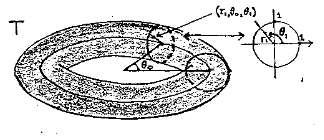
\includegraphics[width=0.5\linewidth]{2.png}
\end{figure}

\noindent If we represent points of a solid torus $T$ with meridianal radius 1, where $\theta_0$ gives the longitudinal position and $\theta_1,r_1$ give the position of the point within the cross-section determined by $\theta_0$, as shown above, then condition $1$ is satisfied, since all angles are identified on a circle with no radius.\\

\noindent The case where $r_1=1$ corresponds to the boundary of $T$. Varying $\theta_0$ then traces out a latitude, so condition $2$ corresponds to identifying each latitude of $\partial T$ with a single point.\\

\noindent T is homeomorphic to a solid cylinder with the ends identified, and identifying each vertical line on the boundary then gives $S^3$ due to satisfying condition $2$. Collapsing the vertical lines to points midway along the cylinder then shows that $S^3$ is homeomorphic to a solid ball with upper and lower hemisphered identified via orthogonal projection, where the lines collapsed to points on the equator, as shown below.\\
\begin{figure} [hbt!]
    \centering
    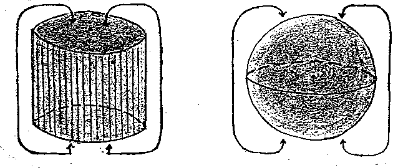
\includegraphics[width=0.5\linewidth]{3.png}
\end{figure}

\noindent To find a geometric model of $L(p;q)$ via identifications on $T$, we much first determine the equivalence classes of the action on $T$. We have that the action of $[m]\in\mathbb{Z}_p$ is given by \[m\cdot(z_0,z_1)=(z_0e^{\frac{2\pi im}{p}},z_1e^{\frac{2\pi iqm}{p}})=(r_0e^{i(\theta_0+\frac{2\pi m}{p})},r_1e^{i(\theta_1+\frac{2\pi qm}{p})}).\] In terms of the coordinates given to $T$, we have\[m\cdot(r,\theta_0,\theta_1)=(r,\theta_0+\frac{2\pi m}{p},\theta_1+\frac{2\pi qm}{p}).\] Note that $r$ is unaffected by the action, meaning that $\mathbb{Z}_p$ maps an individual torus to itself. We can thus express $T$ as\[\bigcup_{0\leq c\leq 1}T_c,\] where $T_c$ is a torus of radius $r$, and study the action on $T$ in terms of the actions on indivudual $T_c$'s.
For the case $0<c<1$, $T_c$ can be pictured as a square with identified edges, with the horizontal axis acting as the $\theta_1$--axis and the vertical axis as the $\theta_0$--axis, both ranging from $0$ to $2\pi$, as shown below:
\begin{figure}[hbt!]
    \centering
    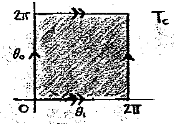
\includegraphics[width=0.5\linewidth]{4.png}
\end{figure}


\noindent The action of $[m]$ on a point $(\theta_0,\theta_1)$ results in the point $(\theta_0+\frac{2\pi m}{p},\theta_1+\frac{2\pi qm}{p})$, so all actions of $\mathbb{Z}_p$ are translations along lines with gradient $\frac{2\pi m}{p}/\frac{2\pi qm}{p}=\frac{1}{q}$. If we divide the square into $p$ horizontal bands, each of height $\frac{2\pi}{p}$, we see that an equivalence class of the action on $T_c$ contains exactly one point in each horizontal band. We can thus define the orbit space as \[T_c/\mathbb{Z}_p=\{(r,\theta_0,\theta_1):r=c,0\leq\theta_0<\frac{2\pi}{p},0\leq\theta_1<2\pi\}.\] This is a short tube with ends identified by a $\frac{2\pi q}{p}$ twist:

\begin{figure} [hbt!]
    \centering
    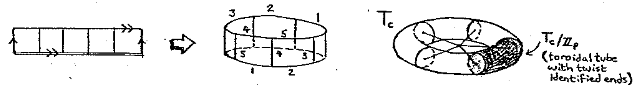
\includegraphics[width=0.5\linewidth]{6.png}
\end{figure}


\noindent We now consider the case $T_0$ - the action on the central circle:\\
The action of $[m]$ on a point in $T_0$ maps $\theta_0$ to $\theta_0+\frac{2\pi m}{p}$, and so $m$ acts by a $\frac{2\pi m}{p}$ rotation. Each equivalence class of the action on $T_0$ thus contains exactly one point in each $\frac{2\pi}{p}$ arc. $0\leq\theta_0<\frac{2\pi}{p}$ thus has exactly one point from each equivalence class, so $T_0/\mathbb{Z}_p$ can be viewed as an arc with identified endpoints.\\

\noindent Finally we consider the case $T_1$ - the boundary of $T$ with each latitude identified to a point:\\
Since $T_1$ is represented by a single meridian of $\partial T$, we can identify $T_1$ with a circle $S^1$. The action of $[m]$ on a point of $T_1$ sends $\theta_1$ to $\theta_1+\frac{2\pi qm}{p}$, and so acts by inducing a $\frac{2\pi qm}{p}$ rotation. Since, $\text{gcd}(p,q)=1$, if we partition $S^1$ into $p$ equal arcs $0\leq\theta_1<\frac{2\pi}{p},...,\frac{2(p-1)\pi}{p}\leq\theta_1<2\pi$, then they all get identified.

\noindent We have \[S^3/\mathbb{Z}_p=\bigcup_{0\leq c\leq 1}T_c/\mathbb{Z}_p.\] This is a collection of nested tubes with radii $0\leq r<1$ whose ends are twist-identified by a $\frac{2\pi q}{p}$--radian twist, and a boundary of latitude-segments which are identified to single points, and then identified from $p$ arcs to one.\\

\noindent Collapsing the latitude segments to points then gives a ball whose equator is divided into $p$ equal arcs, all identified together. The upper and lower hemispheres then correspond to the ends of the solid cylinder and so are twist-identified by a $\frac{2\pi q}{p}$ twist.

\begin{figure} [hbt!]
    \centering
    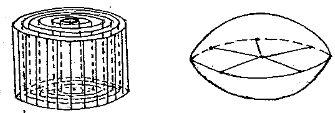
\includegraphics[width=0.5\linewidth]{7.png}
\end{figure}


This then gives a model of $L(p;q)$, which we shall now use to obtain a delta complex.\\





\noindent Consider a filled-in ball with points N and S corresponding to the north and south poles and points $x_0,...,x_{p-1}$ being evenly-spaced points along the equator. Then draw a line through the ball from N to S, lines connecting $x_i$ to $x_{i+1}$, lines connecting $x_i$ to N and lines connecting $x_i$ to S (all geodesic). We then identify the faces on the surface by twisting the top hemisphere by $\frac{2\pi q}{p}$ radians and projecting downwards. This leaves us, after identification, with:\\
Points: $[N]$ and $[x_0]$ (since $\{x_0,x_q,x_{2q},...\}$ are identified and $q$ is coprime to $p$)\\
Lines: $[NS]$, $[x_0x_1]$ and $[Nx_0],...,[Nx_{p-1}]$\\
Faces: $[Nx_0x_1],...,[Nx_{p-2}x_{p-1}],[Nx_0x_{p-1}]$ and $[NSx_0],...,[NSx_{p-1}]$\\
Slices: $[NSx_0x_1],...,[NSx_{p-2}x_{p-1}],[NSx_0x_{p-1}]$.\\
(Here we use $[X]$ to refer to the composition of the quotient map with a singular simplex in the ball and the reason for using $[NSx_0x_{p-1}]$ as opposed to $[NSx_{p-1}x_0]$, for example, is to comply with condition $2$ of the definition of a delta complex)\\

\begin{figure} [hbt!]
    \centering
    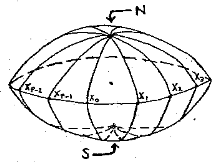
\includegraphics[width=0.5\linewidth]{8.png}
\end{figure}

Having obtained a delta-complex structure, we are now able to compute the torsion linking form of a lens space:
\[\text{Let }a_{p-1}=-[NSx_0x_{p-1}]\text{ and }a_i=[NSx_ix_{i+1}]\text{ otherwise.}\]
\[\text{Let }b_{p-1}=-[Nx_0x_{p-1}]\text{ and }b_i=[Nx_ix_{i+1}]\text{ otherwise.}\]
\[\text{Let }c_i=[NSx_i].\]
\[\text{Let }D=[x_0x_1].\]
\[\text{Let }E=[NS].\]
\[\text{Let }F_i=[Nx_i].\]
\[-\partial b_{p-1}=\partial[Nx_0x_{p-1}]=[x_0x_{p-1}]-[Nx_{p-1}]+[Nx_0]=[Nx_0]-[Nx_{p-1}]-[x_0x_1]\]
Otherwise, \[\partial b_i=\partial[Nx_ix_{i+1}]=[x_0x_1]-[Nx_{i+1}]+[Nx_i]\]
so \[\partial b_i=D-F_{i+1}+F_i.\]
\[\partial c_i=\partial[NSx_i]=[Sx_i]-[Nx_i]+[NS]=[NS]-[Nx_i]+[Nx_{i-q}]\]
so \[\partial c_i=E-F_i+F_{i-q}.\]

\begin{lemma}
$\sum_{i=0}^{p-1}a_i$ is a representative of a fundamental class.
\end{lemma}
\begin{proof}
\[\partial(\sum_{i=0}^{p-1}a_i)=\sum_i([Nx_{i-q}x_{i-q+1}]-[Nx_ix_{i+1}]+[NSx_{i+1}]-[NSx_i])=0\] so $\sum_{i=0}^{p-1}a_i$ is a representative of an element of $H_3(L(p;q);\mathbb{Z})$. The coefficients of $a_i$ are all equal and $H_3(L(p;q);\mathbb{Z})\cong\mathbb{Z}$ so $\sum_{i=0}^{p-1}a_i$ has to represent a generator, and hence a fundamental class.
\end{proof}

Call the equivalence class it represents $[M]$.\\
$C_1(L(p;q),\mathbb{Z})$ has basis $D,E,F_i$ and $C_2(L(p;q),\mathbb{Z})$ has basis $b_i,c_i$.\\
Let $\widehat X$ be linear map which sends $X$ to $1$ and all other elements of the basis to $0$. We then have:\\
\[d\widehat D=\sum_{i=0}^{p-1}\widehat b_i.\]
\[d\widehat E=\sum_{i=0}^{p-1}\widehat c_i.\]
\[d\widehat F_i=\widehat b_i-\widehat b_{i-1}-\widehat c_i+\widehat c_{i+q}.\]
Then define \[\gamma=\widehat D + (\sum_{i=0}^{p-1}i\widehat F_i)+q\widehat E\in C^1(L(p;q);\mathbb{Z}).\]
\begin{align*}
d\gamma&=\sum_{i=0}^{p-1}\widehat b_i+(\sum_{i=0}^{p-1}i(\widehat b_i-\widehat b_{i-1}-\widehat c_i+\widehat c_{i+q}))+\sum_{i=0}^{p-1}q\hat c_i\\
&=\sum_{i=0}^{p-1}((i+1)\widehat b_i-i\widehat b_{i-1}-(i-q)\widehat c_i+i\widehat c_{i+q})\equiv 0\text{ mod }p.
\end{align*}
Let $\alpha=\frac{1}{p}d\gamma\in C^2(L(p;q);\mathbb{Z})$. Then $\alpha$ is a representative of an element in $H^2(L(p;q);\mathbb{Z})$ with $p[\alpha]=[0]$. Also note that $\gamma(E)=q$.
\[p\alpha([Sx_{q-1}x_q])=p\alpha([Nx_{p-1}x_0])=p\alpha(b_{p-1})=(p-1+1)\hat b_{p-1}(b_{p-1})-0\times\hat b_{-1}(b_{p-1})=p\]\[\implies \alpha([Sx_{q-1}x_q])=1.\]
Otherwise, \[p\alpha([Sx_ix_{i+1}])=p\alpha([Nx_{i-q}x_{i+1-q}])=p\alpha(b_{i-q})=(kp+i-q+1)\hat b_{{i-q}}(b_{{i-q}})-(kp+i-q+1)\hat b_{{i-q}}(b_{{i-q}})=0\]where $k\in\mathbb{Z}$ puts $kp+i-q+1$ in the compatible range for the sum of $[1,p-1]$ (The fact that it can't wrap around to $0$ is why cancellation occurs).\\
Thus, \[[\alpha]\vee[\alpha]=\frac{1}{p}\gamma([NS])\alpha([Sx_{q-1}x_q])=\frac{q}{p}.\]

\noindent We then have that if $L(p;q_1)$ and $L(p;q_2)$ are homotopy-equivalent, then $\frac{q_1}{p}=\pm\frac{q_2}{p}m^2$ for some integer $m$, taking into account whether or not the homotopy-equivalence is orientation-reversing and choice of element of $H^2(L(p;q);\mathbb{Z})$ (since $[n\alpha]\vee[n\alpha]=n^2[\alpha]\vee[\alpha]$). This is equivalent to $q_1\equiv\pm q_2m^2\text{ mod }p\iff q_1q_2^{-1}\equiv\pm m^2\text{ mod }p\iff q_1q_2\equiv\pm(mq_2)^2\text{ mod } p\iff q_2q_2\equiv\pm n^2\text{ mod } p$, where $n=mq_2$.\\

\noindent If we were only interested in orientation-preserving homotopy-equivalence, then the condition would be $q_2q_2\equiv n^2\text{ mod } p$; and if we were only interested in orientation-reversing homotopy-equivalence, then the condition would be $q_2q_2\equiv- n^2\text{ mod } p$.
Thus $L(p;q)$ is orientation-reversing homotopy-equivalent to itself iff $q(-q)$ is a square mod $p$ $\iff -1$ is a square mod $p\iff p\equiv 1$ mod $4$ for $p$ a prime. This in contrast to compact $2$--manifolds, which always admit orientation-reversing homeomorphisms.\\

\noindent The proof of the sufficiency of this condition is given in exercise 29 in section 4.2 of Hatcher.



\subsection{Reidemeister torsion}

\begin{definition}\cite{torsion}
Let $0\to C_n\overset{\partial}{\to}C_{n-1}\overset{\partial}{\to}C_{n-2}\overset{\partial}{\to}...\overset{\partial}{\to}C_{0}\to 0$ be a chain complex with coefficients in a commutative ring and with no homology and bases $c_i$ of $C_i$. We can then pick auxiliary bases $b_i\cup\overset{\sim}{b}_{i-1}$ of $C_i$ where $b_i$ is a basis for $\text{Im }\partial_{i+1}$ and $\partial\overset{\sim}{b}_{i-1}=b_{i-1}$. Then let $[b_i\cup\overset{\sim}{b}_{i-1}|c_i]$ be the determinant of the change of basis matrix from $b_i\cup\overset{\sim}{b}_{i-1}$ to $c_i$. We then define The \textbf{Reidemeister torsion} \[\Delta(C_.,c_.)=\prod_{i=0}^n[b_i\cup\overset{\sim}{b}_{i-1}|c_i]^{(-1)^i}.\]
\end{definition}

\begin{theorem}
The Reidemeister torsion is independent of choice of auxiliary bases but not of choice of $c_i$.
\end{theorem}

\noindent Let \[X=\bigcup_{k=0}^n\bigcup_je_j^k\] be a finite cell complex and $(A,\beta)$ a representation of $\pi_1(X)$ in a ring $A$. Let $\overset{\sim}{X}$ be a universal cover. And $\overset{\sim}{e}_j^k$ be a lift of $e_j^k$. Then every other lift of $e_j^k$ is obtained by composition of $\overset{\sim}{e}_j^k$ with a deck transformation (since given $f'$ and $g'$ lifts of $f$ there exists a $\phi\in\text{Aut}(p)$ such that $\phi\circ f'(0)=g'(0)$ which implies $\phi\circ f=g$ by uniqueness). $\text{Aut}(p)=\pi_1(X)$ so we can write \[\overset{\sim}{X}=\bigcup_{k=0}^n\bigcup_{g\in\pi_1(X)}\bigcup_jg\overset{\sim}{e}_j^k.\] Thus multiplication by an element of $\pi_1(x)$ permutes the cells, thereby giving $CC_.(\overset{\sim}{X})$ a $\pi_1(X)$-action. $A$ also has a $\pi_1(X)$ action so we can define $C_k(X;\beta)=CC_k(\overset{\sim}{X})\otimes_{\mathbb{Z}\pi_1(X)} A$, where $\mathbb{Z}\pi_1(X)$ is the free group generated by $\pi_1(X)$. We have an induced boundary map $\partial\colon C_k(X;\beta)\to C_{k-1}(X;\beta)$ which makes $C_k(X;\beta)$ a chain complex with basis $\{\overset{\sim}{e}_j^k\}\otimes\text{id}_A$.

\begin{definition}
If $C_.(X;\beta)\otimes_{\mathbb{Z}\pi_1(X)}A$ has no homology, then the \textbf{Reidemeister torsion of $X$ with respect to $\beta$} is \[\Delta(X;\beta):=\Delta(C_.(X;\beta)\otimes_{\mathbb{Z}\pi_1(X)}A).\] This is a well-defined element of $A^*/\{\pm\beta(\pi_1(X))\}$.
\end{definition}
\begin{remark}
The ambiguity which required modding out by $\{\pm\beta(\pi_1(X))\}$ to solve arose out of the choice of lifts which form the bases $c_i$ -- the choice of which, unlike that of auxiliary bases, $\Delta(C_.,c_.)$ is not independent.
\end{remark}

\begin{theorem}
Let $X$ and $Y$ be cell complexes, let $f:X\to Y$ be a homeomorphism and let $(A,\beta)$ be a representation of $\pi_1(Y)$. Then $\Delta(X;\beta\circ f_*)=\Delta(Y;\beta)$
\end{theorem}

\noindent Thus the Reidemeister torsion is invariant under homeomorphism. However, it is not invariant under homotopy-equivalence. We shall now compute the Reidemeister torsion of a lens space.\\

\subsection{Homeomorphism classification}

\noindent We shall now realise lens spaces as cell complexes, in preparation for computing the Reidemeister torsion to give a stronger homeomorphism invariant than the fundamental group.\\

\cite{lecture}
\noindent We have
\[L(p;q)=\{(r_1e^{2\pi i\theta_1},r_2e^{2\pi i\theta_2}):r_1^2+r_2^2=1\}/(\theta_1,\theta_2)\sim(\theta_1+\frac{1}{p},\theta_2+\frac{q}{p}).\]

\noindent Let $\rho\colon S^3\to S^3$ represent the action.

\noindent The action rotates the first coordinate by $1/p$ so let \[e_k^3=\{(r_1e^{2\pi i\theta_1},r_2e^{2\pi i\theta_2})\in S^3:\frac{k}{p}<\theta_1<\frac{k+1}{p}\}.\]

\noindent The $2$-cells will then be the boundaries of the $3$-cells, so let \[e_k^2=\{(r_1e^{2\pi i\theta_1},r_2e^{2\pi i\theta_2})\in S^3:\theta_1=\frac{k}{p}\}.\]

\noindent Fixing $\theta_1$ leaves $r_2e^{2\pi i\theta_2}$ moving in a circle, so let \[e_k^1=\{(r_1e^{2\pi i\theta_1},r_2e^{2\pi i\theta_2})\in S^3:\theta_1=0,\frac{k}{p}<\theta_2<\frac{k+1}{p}\}.\]

\noindent Then let $e_k^0=\{(r_1e^{2\pi i\theta_1},r_2e^{2\pi i\theta_2})\in S^3:\theta_1=0,\theta_2=\frac{k}{p}\}$ be the boundary of $e_k^1$.

\noindent Then we have $\rho(e_k^3)=e_{k+1}^3$, $\rho(e_k^2)=e_{k+1}^2$, $\rho(e_k^1)=e_{k+q}^1$ and $\rho(e_k^0)=e_{k+q}^0$.

\noindent Thus $\rho$ permutes the cells so taking the quotient gives a cell complex structure \[L(p;q)=e^0\cup e^1\cup e^2\cup e^3.\]

\[\partial e_0^3=e_1^2-e_0^2=(\rho-\text{id})(e_0^2)\]
\[\partial e_1^2=e_0^1+...+e_{p-1}^1=(\text{id}+\rho+...+\rho^{p-1})(e_0^1)\]
\[\partial e_0^1=e_l^0-e_0^0=(\rho^l-\text{id})(e_0^0)\] where $lq\cong1\text{ mod }p$ (so that $l$ corresponds to rotating by $\frac{2\pi i}{p}$).

\noindent Thus on $L(p;q)$, we have $\partial e^3=0$, $\partial e^2=pe^1$, $\partial e^1=0$ since $p=\text{id}$ modulo the group action. This then gives the same homology groups as were found earlier.\\

\noindent Let $\omega$ be a $p$th root of unity and let $\beta_\omega\colon\mathbb{Z}_p\to \mathbb{C}^*$ be the representation given by $1\mapsto\omega$.
In $C_.(X;\beta_\omega)\otimes_{\mathbb{Z}\pi_1(X)}\mathbb{C}^*$ we have:\\
\[\partial(\overset{\sim}{e}_0^3\otimes\text{id})=(\omega-1)(\overset{\sim}{e}_0^2\otimes\text{id}),\]
\[\partial(\overset{\sim}{e}_0^2\otimes\text{id})=(1+\omega+\omega^2+...+\omega^{p-1})(\overset{\sim}{e}_0^1\otimes\text{id}),\]
\[\partial(\overset{\sim}{e}_0^1\otimes\text{id})=(\omega^l-1)(\overset{\sim}{e}_0^0\otimes\text{id}),\] giving a complex:
\[0\to\mathbb{C}^*\overset{\omega-1}{\to}\mathbb{C}^*\overset{0}{\to}\mathbb{C}^*\overset{\omega^l-1}{\to}\mathbb{C}^*\to0\text{ whenever }\omega\neq 1.\]
The non-zero maps are isomorphisms and so the complex has no homology. Hence for $\omega\neq 1$ we have \[\Delta(L(p;q);\beta_\omega)=(\omega^l-1)(\omega-1)\in\mathbb{C}^*/\{\pm\omega^k:k\in\mathbb{Z}\}.\]
\[(\omega^l-1)(\omega-1)=\omega^l(1-\omega^{-l})(\omega-1)=(\omega^{-l}-1)(\omega-1)=\omega(\omega^{-l}-1)(1-\omega^{-1})=(\omega^{-l}-1)(\omega^{-1}-1)\] so \[\Delta(L(p;q);\beta_\omega)=\Delta(L(p;-q);\beta_{\omega^{-1}}).\]
It can also be shown that \[\Delta(L(p;q);\beta_\omega)=\Delta(L(p;q^{-1});\beta_{\omega^l}).\]
Thus a necessary condition for two lens spaces $L(p;q_1)$ and $L(p;q_2)$ to be homeomorphic is that $q_1\equiv \pm q_2^{\pm 1}\text{mod }p$.\\

\noindent To give the complete homeomorphism classification, we require the following lemma.

\begin{lemma}
Let X be a topological space. Let $G_1$ and $G_2$ be conjugate subgroups of Homeo$(X)$ defining covering space actions of $X$. Then $X/G_1\cong X/G_2$.
\end{lemma}
\begin{proof}
We have that $G_2=hG_1h^{-1}$ for some $h\in\text{Homeo}(X)$. The map $f:X\to X/G_2\colon x\mapsto[h\cdot y]$ is continuous, since $h$ acts by a homeomorphism and the quotient map is continuous. We also have that if $x'=g_1\cdot y$ for some $g_1\in G_1$, then \[f(x')=[hg_1\cdot x]=[(hg_1^{-1}h^{-1})\cdot hg_1\cdot x]=[h\cdot x]=f(x).\] The universal property of quotient maps then implies that there exists a continuous map $\bar f:X/G_1\to X/G_2$. Similarly, there exists a continuous map $\bar g:X/G_2\to X/G_1\colon [x]\mapsto[h^{-1}\cdot x]$. \[\bar g\circ\bar f([x])=[h^{-1}\cdot (h\cdot x)]=[x].\] Similarly, $\bar f\circ\bar g([x])=[x]$. Thus $X/G_1\cong X/G_2$.
\end{proof}

\begin{lemma}
$L(p;q)\cong L(p;-q)$.
\end{lemma}
\begin{proof}
$(v,w)\mapsto(e^{2\pi i/p}v,e^{2\pi iq/p}w)$ and $(v,w)\mapsto(e^{2\pi i/p}v,e^{-2\pi iq/p}w)$ are conjugate by the homeomorphism $(v,w)\mapsto(v,\bar w)$. The result follows by the above lemma.
\end{proof}
\begin{lemma}
If $q_1\equiv q_2^{-1}\text{ mod }p$ then $L(p;q_1)\cong L(p;q_2)$.
\end{lemma}
\begin{proof}
We have that $q_1q_2\equiv 1\text{ mod }p$.
\[{(e^{2i\pi/p})}^{q_1}=e^{2i\pi q_1/p},{(e^{2i\pi/p})}^{q_2}=e^{2i\pi q_2/p}\] and \[{(e^{2i\pi q_1/p})}^{q_2}=e^{2i\pi /p}={(e^{2i\pi q_2/p})}^{q_1}.\] Thus the subgroup generated by \[(v,w)\mapsto(e^{2i\pi /p}v,e^{2i\pi q_1/p}w)\] is the same as the subgroup generated by \[(v,w)\mapsto(e^{2i\pi q_2/p}v,e^{2i\pi/p}w).\] Furthermore, \[(v,w)\mapsto(e^{2i\pi q_2/p}v,e^{2i\pi/p}w)\] is conjugate to \[(v,w)\mapsto(e^{2i\pi/p}w,e^{2i\pi q_2/p}v)\] by the homeomorphism $(v,w)\mapsto(w,v)$. Thus the subgroups generated by \[(v,w)\mapsto(e^{2i\pi /p}v,e^{2i\pi q_1/p}w)\] and \[(v,w)\mapsto(e^{2i\pi /p}v,e^{2i\pi q_2/p}w)\] are conjugate so $L(p;q_1)\cong L(p;q_2)$.
\end{proof}

\noindent This completes the homeomorphism classification.

\begin{theorem}
Let $L(p;q_1)$ and $L(p;q_2)$ be lens spaces.\\
They are homotopy equivalent if and only if $q_1q_2\equiv\pm n^2 \text{ mod } p$ for some $n\in\mathbb{N}$.\\
They are homeomorphic if and only if $q_1\equiv\pm q_2^{\pm 1} \text{ mod }p$.
\end{theorem}

\begin{example}
$L(7;1)$ and $L(7;2)$ are homotopy-equivalent but not homeomorphic.
\end{example}
\noindent This is significant, since it gives a counter-example to a once-believed conjecture that homotopy-equivalent and homeomorphic are equivalent conditions for manifolds.

\bibliographystyle{IEEEtran}
\bibliography{sources.bib}

\end{document}

